\documentclass[twocolumn,10pt]{article}

\usepackage[margin=1.8cm]{geometry}
\usepackage{amsmath, amssymb}
\usepackage{graphicx}
\usepackage{physics}
\usepackage{bm}
\usepackage{authblk}
\setlength{\columnsep}{0.6cm}

%\title{\textbf{Entanglement-Dynamic Topology Enables Programmable Quantum Resources}}
% ============================================================
% TITLE
% ============================================================

\title{
Programmable Quantum Resource Manifolds via Entanglement-Dynamic Topology
}

\author[1]{Hang Hu \thanks{Correspondence to: hang.hu@cnrc-nrc.gc.ca}}
\affil[1]{Digital Technologies, National Research Council of Canada, 222 College Street, Toronto, ON M5T 3J1, Canada}
\author[1]{Hsu Kiang Ooi}
\author[2]{Anguang Hu \thanks{Correspondence to: anguang.hu@forces.gc.ca}}
\affil[2]{Suffield Research Centre, Defence Research and Development Canada, PO Box 4000 Station Main, Medicine Hat, Alberta T1A 8K6, Canada}

\date{\today}

\begin{document}

\twocolumn[
\maketitle
\begin{center}
\small
Correspondence to: hang.hu@cnrc-nrc.gc.ca; anguang.hu@forces.gc.ca
\end{center}
\vspace{0.5em}
\begin{center}
\begin{minipage}{0.95\textwidth}
\small
\textbf{Abstract.}
Quantum technologies rely on entanglement, coherence, superposition, and interference as fundamental resources, yet conventional approaches seek to maximize these quantities globally, leading to exponential complexity associated with Hilbert-space scaling. Here we introduce Entanglement–Dynamic Topology (EDT) as a framework for programmable quantum resource engineering, in which quantum resources are organized into finite, geometry-aligned manifolds rather than distributed across the full Hilbert space. We show that EDT emerges from non-adiabatic coupling between electronic and lattice degrees of freedom, where second-order variations of electronic energies with respect to normal-mode coordinates generate curvature fields that act as sources of entanglement and organize interference through geometric and topological structure. This connects EDT directly to the microscopic physics of electron–phonon interactions, including the Bardeen–Pines formalism and the foundations of BCS theory. We demonstrate a data-driven identification of EDT in K$_3$C$_{60}$, where curvature-resolved band structure reveals a finite momentum interval in which paired branches admit a consistent local quadratic description. We further show that this regime emerges generically in a minimal dynamical model, where loop-induced operator spreading remains structured and compatible with persistent many-body correlations, and that it is robust under parameter variation, bounded circuit complexity, and approximate implementation. Finally, we establish an experimental realization in NV-center sensing, where optimal performance arises within a finite control regime balancing competing quantum resources. These results establish a new paradigm in which quantum advantage arises not from Hilbert-space scaling, but from the controlled organization of quantum resources into structured dynamical manifolds generated by microscopic interactions.
\end{minipage}
\end{center}
\vspace{1em}
]

% ============================================================
%\begin{abstract}
%Quantum technologies rely on entanglement, coherence, superposition, and interference as fundamental resources, yet conventional approaches seek to maximize these quantities globally, leading to exponential complexity associated with Hilbert-space scaling. Here we introduce Entanglement–Dynamic Topology (EDT) as a framework for programmable quantum resource engineering, in which quantum resources are organized into finite, geometry-aligned manifolds rather than distributed across the full Hilbert space. We show that EDT emerges from non-adiabatic coupling between electronic and lattice degrees of freedom. In this picture, second-order variations of electronic energies with respect to normal-mode coordinates generate curvature fields that act as sources of entanglement and organize interference through geometric and topological structure. This connects EDT directly to the microscopic physics of electron–phonon interactions, including the Bardeen–Pines formalism and the foundations of BCS theory. We demonstrate a data-driven identification of EDT in K$_3$C$_{60}$, where curvature-resolved band structure reveals a finite momentum interval in which paired branches admit a consistent local quadratic description. We then show that this regime emerges generically in a minimal dynamical model, where loop-induced operator spreading remains structured and compatible with persistent many-body correlation, and that it remains robust under parameter variation, bounded circuit complexity, and approximate implementation. Finally, we establish an experimental realization in NV-center sensing, where optimal performance arises within a finite control regime balancing competing quantum resources. These results establish a new paradigm in which quantum advantage arises from the organization of quantum resources into structured dynamical manifolds generated by microscopic interactions, with implications for quantum computing, sensing, and superconducting materials.
%\end{abstract}
%\setlength{\parskip}{0pt}
%\begin{abstract}\noindent
%Quantum technologies rely on entanglement, coherence, superposition, and interference as fundamental resources, yet conventional approaches seek to maximize these quantities globally, leading to exponential complexity associated with Hilbert-space scaling. Here we introduce Entanglement–Dynamic Topology (EDT) as a framework for programmable quantum resource engineering, in which quantum resources are organized into finite, geometry-aligned manifolds rather than distributed across the full Hilbert space. We show that EDT emerges from non-adiabatic coupling between electronic and lattice degrees of freedom, where second-order variations of electronic energies with respect to normal-mode coordinates generate curvature fields that act as sources of entanglement and organize interference through geometric and topological structure. This connects EDT directly to the microscopic physics of electron–phonon interactions, including the Bardeen–Pines formalism and the foundations of BCS theory. We demonstrate a data-driven identification of EDT in K$_3$C$_{60}$, where curvature-resolved band structure reveals a finite momentum interval in which paired branches admit a consistent local quadratic description. We further show that this regime emerges generically in a minimal dynamical model, where loop-induced operator spreading remains structured and compatible with persistent many-body correlations, and that it is robust under parameter variation, bounded circuit complexity, and approximate implementation. Finally, we establish an experimental realization in NV-center sensing, where optimal performance arises within a finite control regime balancing competing quantum resources. These results establish a new paradigm in which quantum advantage arises not from Hilbert-space scaling, but from the controlled organization of quantum resources into structured dynamical manifolds generated by microscopic interactions.
%\end{abstract}

% ============================================================
\section*{Introduction}

%Quantum computation, sensing, and materials design fundamentally depend on the controlled use of quantum resources, including entanglement, coherence, superposition, and interference. In most current approaches, these resources are treated as quantities to be maximized, leading naturally to strategies that explore increasingly large Hilbert spaces. While powerful in principle, this paradigm introduces severe scaling challenges and often obscures the physical structure underlying useful quantum dynamics.

%An alternative perspective is that quantum advantage arises not from the size of Hilbert space, but from the \emph{organization} of quantum resources within it. In this view, the central problem is not to generate maximal entanglement, but to engineer entanglement that is structured, localized, and aligned with the geometry of the task. This shift reframes quantum control as a problem of resource organization rather than resource amplification. In this sense, useful quantum dynamics are not those that explore the largest possible state space, but those that remain confined to structured manifolds where entanglement, interference, and correlation are jointly optimized.

Quantum computation, sensing, and materials design fundamentally depend on the controlled use of quantum resources, including entanglement, coherence, superposition, and interference~\cite{NielsenChuang,Horodecki2009,Streltsov2017}. In most current approaches, these resources are treated as quantities to be maximized, leading naturally to strategies that explore increasingly large Hilbert spaces~\cite{Preskill2018,Arute2019}. While powerful in principle, this paradigm introduces severe scaling challenges and often obscures the physical structure underlying useful quantum dynamics~\cite{Eisert2010,Altman2015}.

An alternative perspective is that quantum advantage arises not from the size of Hilbert space, but from the \emph{organization} of quantum resources within it~\cite{Amico2008,Swingle2018}. In this view, the central problem is not to generate maximal entanglement, but to engineer entanglement that is structured, localized, and aligned with the geometry of the task~\cite{Verstraete2008,Orus2014}. This shift reframes quantum control as a problem of resource organization rather than resource amplification. In this sense, useful quantum dynamics are not those that explore the largest possible state space, but those that remain confined to structured manifolds where entanglement, interference, and correlation are jointly optimized~\cite{KimHuse2013,Choi2016}.

%Here we introduce Entanglement–Dynamic Topology (EDT) as a unifying framework for programmable quantum resource engineering. EDT describes a regime of quantum dynamics in which resources are simultaneously \emph{structured, interacting, topological, and dynamical}. As illustrated in Fig.~\ref{fig:edt_concept}, these four elements play complementary roles. Structure, arising from symmetry, constrains quantum states into reduced manifolds. Interaction, driven by non-adiabatic coupling such as electron–phonon interaction, generates and redistributes entanglement. Topology organizes this structure through nodes, poles, and vortex-like configurations in parameter space. Dynamics, through modulation of band energies and electronic potentials, renders these manifolds controllable and programmable. Together, these elements define a regime in which quantum resources are structured by symmetry, generated by interaction, organized by topology, and controlled by dynamics.

%A key feature of EDT is that it defines a \emph{finite regime} rather than a fine-tuned point. Within this regime, quantum dynamics exhibit coherent, structured behavior, while outside it the dynamics become either weakly correlated or overdriven and incoherent. This regime-based perspective provides a robust and experimentally meaningful foundation for quantum resource engineering, in contrast to approaches that rely on asymptotic scaling or finely tuned optimality.

%To connect this framework to real physical systems, we first develop a data-driven method for identifying EDT directly from electronic structure observables. Using K$_3$C$_{60}$ as a representative system, we analyze curvature-resolved band structure and show that EDT emerges as a finite momentum interval in which paired curvature branches admit a consistent local quadratic description (Fig.~2). This provides an operational criterion for detecting EDT and establishes a direct link between microscopic electronic structure and structured quantum resources.

%We then show that this regime arises generically in a minimal dynamical model (Fig.~3), where loop-induced operator spreading remains structured and compatible with persistent many-body correlation, and that it remains robust under parameter variation, bounded circuit complexity, and approximate implementation (Fig.~4). These results demonstrate that EDT is not a material-specific phenomenon, but a general dynamical principle that connects microscopic physics, quantum dynamics, and practical implementation.

%More broadly, EDT enables a programmable resource paradigm in which target quantum resources are mapped onto finite manifolds and compiled into physical control primitives. This shifts the focus of quantum science from Hilbert-space scaling to resource structuring, with implications for quantum computing, sensing, and geometry-aligned algorithm design.

Here we introduce Entanglement–Dynamic Topology (EDT) as a unifying framework for programmable quantum resource engineering, building on recent developments in curvature-driven and topologically structured quantum dynamics~\cite{Hu2024_ACP,Hu2025_APQ,Hu2026_JPCM}. EDT describes a regime of quantum dynamics in which resources are simultaneously \emph{structured, interacting, topological, and dynamical}. As illustrated in Fig.~\ref{fig:edt_concept}, these four elements play complementary roles. Structure, arising from symmetry, constrains quantum states into reduced manifolds~\cite{Wigner1959,Georgi1999}. Interaction, driven by non-adiabatic coupling such as electron–phonon interaction, generates and redistributes entanglement~\cite{Mead1979,Yarkony1996}. Topology organizes this structure through nodes, poles, and vortex-like configurations in parameter space~\cite{Berry1984,Xiao2010}. Dynamics, through modulation of band energies and electronic potentials, renders these manifolds controllable and programmable~\cite{Bukov2015,Eckardt2017}. Together, these elements define a regime in which quantum resources are structured by symmetry, generated by interaction, organized by topology, and controlled by dynamics.

A key feature of EDT is that it defines a \emph{finite regime} rather than a fine-tuned point. Within this regime, quantum dynamics exhibit coherent, structured behavior, while outside it the dynamics become either weakly correlated or overdriven and incoherent~\cite{Larkin1969,Swingle2018}. This regime-based perspective provides a robust and experimentally meaningful foundation for quantum resource engineering, in contrast to approaches that rely on asymptotic scaling or finely tuned optimality.

To connect this framework to real physical systems, we first develop a data-driven method for identifying EDT directly from electronic structure observables. Using K$_3$C$_{60}$ as a representative system, we analyze curvature-resolved band structure and show that EDT emerges as a finite momentum interval in which paired curvature branches admit a consistent local quadratic description (Fig.~2). This provides an operational criterion for detecting EDT and establishes a direct link between microscopic electronic structure and structured quantum resources~\cite{Gunnarsson1997,Capone2009}.

We then show that this regime arises generically in a minimal dynamical model (Fig.~3), where loop-induced operator spreading remains structured and compatible with persistent many-body correlation, and that it remains robust under parameter variation, bounded circuit complexity, and approximate implementation (Fig.~4)~\cite{Lloyd1996,Childs2019}. These results demonstrate that EDT is not a material-specific phenomenon, but a general dynamical principle that connects microscopic physics, quantum dynamics, and practical implementation.

More broadly, EDT enables a programmable resource paradigm in which target quantum resources are mapped onto finite manifolds and compiled into physical control primitives. This shifts the focus of quantum science from Hilbert-space scaling to resource structuring, with implications for quantum computing, sensing, and geometry-aligned algorithm design~\cite{Preskill2018,Verstraete2008}.

% ============================================================
% SECTION II
% ============================================================
%\section*{Physical Origin and Organization of Entanglement-Dynamic Topology}

%EDT emerges from the interplay of symmetry, interaction, topology, and dynamics in quantum systems, providing a physical mechanism by which quantum resources become structured, localized, and operationally accessible. Rather than treating entanglement, coherence, superposition, and interference as globally distributed quantities, EDT identifies a regime in which these resources arise from physically constrained processes and are organized within finite manifolds in Hilbert space.

%As illustrated in Fig.~\ref{fig:edt_concept}, the origin of EDT begins with symmetry, which imposes a fundamental organization on quantum states. Symmetry decomposes Hilbert space into constrained manifolds, restricting dynamics to geometry-aligned subspaces (Fig.~\ref{fig:edt_concept}B). This structural reduction concentrates quantum resources into physically meaningful sectors, replacing uniform Hilbert-space exploration with a structured resource landscape. In this sense, symmetry defines the geometric scaffold on which quantum dynamics unfold.

%Interactions provide the mechanism for generating and redistributing quantum resources within this scaffold. In particular, non-adiabatic coupling, such as electron--phonon interaction, induces mixing between electronic states through nuclear motion. As shown schematically in Fig.~\ref{fig:edt_concept}A, near degeneracies and band crossings act as curvature sources, where second-order variations of band energies generate strong coupling. Unlike adiabatic descriptions, which treat electronic states as isolated, these non-adiabatic processes dynamically generate entanglement, enabling correlated quantum states that extend across the structured manifold.

%The combination of symmetry and interaction gives rise to a topological organization of quantum resources. Near degeneracies and avoided crossings, non-adiabatic coupling fields develop geometric features in parameter space, including nodes, poles, and vortex-like structures. These features act as organizing centers for quantum dynamics, stabilizing interference and defining pathways along which quantum resources are concentrated and transported (Fig.~\ref{fig:edt_concept}B). In this way, topology provides a robust geometric framework that governs how entanglement and coherence are distributed.

%Crucially, these structures are not static. Time-dependent modulation of band energies and electronic potentials renders the resource manifold dynamical and controllable. External drives, lattice distortions, or environmental interactions can shift and reshape the manifold, enabling the preparation, steering, and stabilization of quantum resources. This dynamical aspect transforms the structured manifold into a programmable object, allowing quantum resources to be engineered through physically accessible control parameters (Fig.~\ref{fig:edt_concept}C).

%These physical ingredients naturally define a computational and operational framework. As shown in Fig.~\ref{fig:edt_concept}C–E, the structured manifold can be compiled into symmetry-adapted architectures, such as Schur-sector decompositions, Clebsch–Gordan coupling trees, and tensor-network representations, enabling Hilbert-space compression and task-relevant pathway concentration. Rather than uniformly sampling the full operator space, EDT-aligned strategies restrict dynamics to physically relevant sectors, enhancing efficiency and interpretability.

%The same principle extends to sensing and measurement. As illustrated in Fig.~\ref{fig:edt_concept}F, structured manifolds enable selective response and coherence localization in quantum sensors, such as NV-center platforms, where external fields couple preferentially to EDT-aligned modes. This provides a route to enhanced sensitivity without sacrificing coherence through overdriven dynamics.

%Together, these elements define a finite regime of EDT. Within this regime, symmetry constrains accessible states, interaction generates entanglement, topology organizes the resulting structure, and dynamics enables control. The result is a localized, stable, and geometry-aligned manifold in which quantum resources are concentrated and directly usable. Outside this regime, the structure breaks down: dynamics either remain weakly correlated or become overdriven and incoherent.

%This perspective establishes a shift from Hilbert-space scaling to resource organization as the central principle of quantum functionality. EDT identifies the physical origin of usable quantum resources as arising from structured, interacting, topological, and dynamical processes, providing a unified framework that connects microscopic quantum physics to programmable quantum technologies.

\section*{Physical Origin and Organization of Entanglement-Dynamic Topology}

%Entanglement--Dynamic Topology (EDT) emerges from the interplay of symmetry, interaction, topology, and dynamics in quantum systems, providing a physical mechanism by which quantum resources become structured, localized, and operationally accessible. Rather than treating entanglement, coherence, superposition, and interference as globally distributed quantities, EDT identifies a regime in which these resources arise from physically constrained processes and are organized within finite, geometry-aligned manifolds in Hilbert space.

%As illustrated in Fig.~\ref{fig:edt_concept}, the origin of EDT begins with symmetry, which imposes a fundamental organization on quantum states. Symmetry decomposes Hilbert space into constrained manifolds, restricting dynamics to geometry-aligned subspaces (Fig.~\ref{fig:edt_concept}B). This structural reduction concentrates quantum resources into physically meaningful sectors, replacing uniform Hilbert-space exploration with a structured resource landscape. In this sense, symmetry defines the geometric scaffold on which quantum dynamics unfold.

%Interactions provide the mechanism for generating and redistributing quantum resources within this scaffold. In particular, non-adiabatic coupling (NACT), such as electron--phonon interaction, induces mixing between electronic states through nuclear motion. Near degeneracies and band crossings, this mixing becomes enhanced, giving rise to strong second-order modulation of band energies. These effects are captured by the curvature
%\begin{equation}
%\kappa_{n\alpha} = \frac{\partial^2 E_n}{\partial Q_\alpha^2},
%\end{equation}
%which quantifies the response of electronic structure to lattice motion and serves as a microscopic source of entanglement. Unlike adiabatic descriptions, which treat electronic states as isolated, these non-adiabatic processes dynamically generate correlated quantum states that extend across the structured manifold.
%
%The combination of symmetry and interaction gives rise to a topological organization of quantum resources. The NACT fields
%\begin{equation}
%A^{(\alpha)}_{mn} = \langle m | \partial_{Q_\alpha} | n \rangle
%\end{equation}
%define a Berry-like connection in parameter space, whose associated curvature encodes the geometric structure of the coupled electronic manifold. Near degeneracies, this structure manifests as nodes, poles, and vortex-like features that act as organizing centers for quantum dynamics, stabilizing interference and defining pathways along which quantum resources are concentrated and transported (Fig.~\ref{fig:edt_concept}B).
%
%Crucially, these structures are dynamical. Time-dependent modulation of band energies and electronic potentials renders the resource manifold controllable. External drives, lattice distortions, and environmental interactions reshape the curvature landscape, enabling preparation, steering, and stabilization of quantum resources (Fig.~\ref{fig:edt_concept}C). This dynamical aspect transforms the structured manifold into a programmable object.
%
%These physical ingredients naturally define an effective description in terms of curvature-mediated interactions. Starting from the electron--phonon Hamiltonian,
%\begin{equation}
%H = H_e(\mathbf{r};\{Q_\alpha\}) + \sum_\alpha \left(\frac{P_\alpha^2}{2M_\alpha} + \frac{1}{2} M_\alpha \omega_\alpha^2 Q_\alpha^2\right),
%\end{equation}
%a second-order expansion in $Q_\alpha$ and projection onto an electronic subspace yields NACT-induced mixing and an effective Hamiltonian of the form
%\begin{equation}
%H_{\mathrm{eff}} \simeq H_0 + \sum_{\langle i,j\rangle} J_{ij}\, Z_i Z_j
%+ \sum_p \lambda_p\, W_p,
%\end{equation}
%where $J_{ij}$ arises from curvature-mediated processes and $W_p$ denotes loop (plaquette) operators generated by multi-mode interference of NACT fields. These loop terms encode the holonomy of the underlying geometric connection and generate structured, non-local entanglement.

%Within this framework, EDT defines a finite regime of dynamics. When curvature is smoothly varying and geometrically coherent, paired structures admit a stable quadratic description, yielding a finite EDT window in which quantum resources are localized and robust. Outside this regime, either curvature is too weak to generate correlations or too sharply varying to support a stable manifold, leading to weakly correlated or overdriven dynamics.

%This perspective establishes a shift from Hilbert-space scaling to resource organization as the central principle of quantum functionality. EDT identifies the physical origin of usable quantum resources as arising from structured, interacting, topological, and dynamical processes, providing a unified framework that connects microscopic quantum physics to programmable quantum technologies.
EDT emerges from the interplay of symmetry, interaction, topology, and dynamics in quantum systems, providing a physical mechanism by which quantum resources become structured, localized, and operationally accessible~\cite{NielsenChuang,Horodecki2009}. Rather than treating entanglement, coherence, superposition, and interference as globally distributed quantities, EDT identifies a regime in which these resources arise from physically constrained processes and are organized within finite, geometry-aligned manifolds in Hilbert space~\cite{Amico2008,Eisert2010}.

As illustrated in Fig.~\ref{fig:edt_concept}, the origin of EDT begins with symmetry, which imposes a fundamental organization on quantum states. Symmetry decomposes Hilbert space into constrained manifolds, restricting dynamics to geometry-aligned subspaces (Fig.~\ref{fig:edt_concept}B)~\cite{Wigner1959,Georgi1999}. This structural reduction concentrates quantum resources into physically meaningful sectors, replacing uniform Hilbert-space exploration with a structured resource landscape. In this sense, symmetry defines the geometric scaffold on which quantum dynamics unfold.

Interactions provide the mechanism for generating and redistributing quantum resources within this scaffold. In particular, non-adiabatic coupling (NACT), such as electron--phonon interaction, induces mixing between electronic states through nuclear motion~\cite{Mead1979,Yarkony1996}. Near degeneracies and band crossings, this mixing becomes enhanced, giving rise to strong second-order modulation of band energies. These effects are captured by the curvature
\begin{equation}
\kappa_{n\alpha} = \frac{\partial^2 E_n}{\partial Q_\alpha^2},
\end{equation}
which quantifies the response of electronic structure to lattice motion and serves as a microscopic source of entanglement. Unlike adiabatic descriptions, which treat electronic states as isolated, these non-adiabatic processes dynamically generate correlated quantum states that extend across the structured manifold~\cite{BornOppenheimer1927}. This curvature-based and topological organization of quantum dynamics has been previously identified in compressed metallic systems and quantum bonding regimes~\cite{Hu2024_ACP,Hu2025_APQ,Hu2026_JPCM}.

The combination of symmetry and interaction gives rise to a topological organization of quantum resources. The NACT fields
\begin{equation}
A^{(\alpha)}_{mn} = \langle m | \partial_{Q_\alpha} | n \rangle
\end{equation}
define a Berry-like connection in parameter space, whose associated curvature encodes the geometric structure of the coupled electronic manifold~\cite{Berry1984,Xiao2010}. Near degeneracies, this structure manifests as nodes, poles, and vortex-like features that act as organizing centers for quantum dynamics, stabilizing interference and defining pathways along which quantum resources are concentrated and transported (Fig.~\ref{fig:edt_concept}B).

%Crucially, these structures are dynamical. Time-dependent modulation of band energies and electronic potentials renders the resource manifold controllable. External drives, lattice distortions, and environmental interactions reshape the curvature landscape, enabling preparation, steering, and stabilization of quantum resources (Fig.~\ref{fig:edt_concept}C)~\cite{Bukov2015,Eckardt2017}. This dynamical aspect transforms the structured manifold into a programmable object.

%These physical ingredients naturally define an effective description in terms of curvature-mediated interactions. Starting from the electron--phonon Hamiltonian,
%\begin{equation}
%H = H_e(\mathbf{r};\{Q_\alpha\}) + \sum_\alpha \left(\frac{P_\alpha^2}{2M_\alpha} + \frac{1}{2} M_\alpha \omega_\alpha^2 Q_\alpha^2\right),
%\end{equation}
%a second-order expansion in $Q_\alpha$ and projection onto an electronic subspace yields NACT-induced mixing and an effective Hamiltonian of the form
%\begin{equation}
%H_{\mathrm{eff}} \simeq H_0 + \sum_{\langle i,j\rangle} J_{ij}\, Z_i Z_j
%+ \sum_p \lambda_p\, W_p,
%\end{equation}
%where $J_{ij}$ arises from curvature-mediated processes and $W_p$ denotes loop (plaquette) operators generated by multi-mode interference of NACT fields. These loop terms encode the holonomy of the underlying geometric connection and generate structured, non-local entanglement~\cite{BardeenPines1955,BCS1957}.
%
%These physical ingredients also naturally define a computational and operational framework. As shown in Fig.~\ref{fig:edt_concept}C–E, the structured manifold can be compiled into symmetry-adapted architectures, such as Schur-sector decompositions, Clebsch–Gordan coupling trees, and tensor-network representations, including angular-momentum-resolved tensor networks (AM-TTN), enabling Hilbert-space compression and task-relevant pathway concentration. Rather than uniformly sampling the full operator space, EDT-aligned strategies restrict dynamics to physically relevant sectors, enhancing efficiency and interpretability.

Crucially, these structures are dynamical. Time-dependent modulation of band energies and electronic potentials renders the resource manifold controllable. External drives, lattice distortions, and environmental interactions reshape the curvature landscape, enabling preparation, steering, and stabilization of quantum resources (Fig.~\ref{fig:edt_concept}C)~\cite{Bukov2015,Eckardt2017}. This dynamical aspect transforms the structured manifold into a programmable object.

These ingredients admit an effective description in terms of curvature-mediated interactions. Starting from the electron--phonon Hamiltonian,
\begin{equation}
H = H_e(\mathbf{r};\{Q_\alpha\}) + \sum_\alpha \left(\frac{P_\alpha^2}{2M_\alpha} + \frac{1}{2} M_\alpha \omega_\alpha^2 Q_\alpha^2\right),
\end{equation}
a second-order expansion in $Q_\alpha$ and projection onto a near-degenerate electronic subspace yields NACT-induced mixing and an effective Hamiltonian of the form
\begin{equation}
H_{\mathrm{eff}} \simeq H_0 + \sum_{\langle i,j\rangle} J_{ij}\, Z_i Z_j
+ \sum_p \lambda_p\, W_p,
\end{equation}
where $J_{ij}$ arises from curvature-mediated processes and $W_p$ denotes loop (plaquette) operators generated by multi-mode interference of NACT fields. These loop terms encode the holonomy of the underlying geometric connection and give rise to structured, non-local entanglement~\cite{BardeenPines1955,BCS1957}.

At the operational level, these structures define a computational framework. As shown in Fig.~\ref{fig:edt_concept}C–E, the structured manifold can be compiled into symmetry-adapted architectures, including Schur-sector decompositions, Clebsch–Gordan coupling trees, and tensor-network representations such as angular-momentum-resolved tensor networks (AM-TTN). These constructions enable Hilbert-space compression and concentration of dynamics along task-relevant pathways. Rather than uniformly sampling the full operator space, EDT-aligned strategies restrict evolution to physically meaningful sectors, enhancing both efficiency and interpretability. These symmetry-resolved constructions are closely related to decoherence-free subspaces and symmetry-protected encodings, where quantum information is confined to invariant sectors of the Hilbert space~\cite{Bacon2006}.

Within this framework, EDT defines a finite regime of dynamics. When curvature is smoothly varying and geometrically coherent, paired structures admit a stable quadratic description, yielding a finite EDT window in which quantum resources are localized and robust. Outside this regime, either curvature is too weak to generate correlations or too sharply varying to support a stable manifold, leading to weakly correlated or overdriven dynamics~\cite{Larkin1969,Swingle2018}.

This perspective establishes a shift from Hilbert-space scaling to resource organization as the central principle of quantum functionality. EDT identifies the physical origin of usable quantum resources as arising from structured, interacting, topological, and dynamical processes, providing a unified framework that connects microscopic quantum physics to programmable quantum technologies.

Importantly, this structure is not limited to materials systems. The same Hamiltonian structure can be implemented in quantum circuits through Trotterized evolution of local interactions and plaquette terms, providing a direct realization of EDT dynamics in gate-based architectures (see Supplementary Information (SI), Sec.~S7)~\cite{Lloyd1996,Childs2019}. This establishes EDT as a unifying framework spanning electronic structure, dynamical topology, and quantum information processing.


%Importantly, this structure is not limited to materials systems. The same Hamiltonian structure can be implemented in quantum circuits through Trotterized evolution of local interactions and plaquette terms, providing a direct realization of EDT dynamics in gate-based architectures (see Supplementary Information (SI), Sec.~S7). This establishes EDT as a unifying framework spanning electronic structure, dynamical topology, and quantum information processing.

%\paragraph*{From non-adiabatic coupling to an effective EDT Hamiltonian.}

%Starting from the electron–phonon Hamiltonian
%\begin{equation}
%H = H_e(\mathbf{r};\{Q_\alpha\}) + \sum_\alpha \left(\frac{P_\alpha^2}{2M_\alpha} + \frac{1}{2} M_\alpha \omega_\alpha^2 Q_\alpha^2\right),
%\end{equation}
%non-adiabatic effects arise from the dependence of the electronic Hamiltonian on normal-mode coordinates $Q_\alpha$. Expanding $H_e$ to second order,
%\begin{equation}
%H_e(\{Q_\alpha\}) \approx H_e^{(0)} + \sum_\alpha Q_\alpha \,\partial_\alpha H_e
%+ \frac{1}{2}\sum_{\alpha\beta} Q_\alpha Q_\beta \,\partial_\alpha \partial_\beta H_e,
%\end{equation}
%and projecting onto an adiabatic electronic basis $\{|n\rangle\}$ yields non-adiabatic coupling (NACT) matrix elements
%\begin{equation}
%A^{(\alpha)}_{mn} = \langle m | \partial_{Q_\alpha} | n \rangle,
%\end{equation}
%which generate off-diagonal mixing and geometric phases. Eliminating fast phonon coordinates (e.g., via a Born–Oppenheimer breakdown or polaron/Schrieffer–Wolff treatment) produces an effective electronic Hamiltonian with curvature-mediated interactions,
%\begin{equation}
%H_{\mathrm{eff}} \simeq H_0 + \sum_{\langle i,j\rangle} J_{ij}\, Z_i Z_j
%+ \sum_p \lambda_p\, W_p,
%\end{equation}
%where $J_{ij}$ arises from second-order (curvature) processes and $W_p$ denotes loop (plaquette) operators generated by multi-mode interference of NACT fields.
%
%In momentum space, the same physics appears as curvature of band energies with respect to normal-mode coordinates,
%\begin{equation}
%\kappa_{n\alpha} = \frac{\partial^2 E_n}{\partial Q_\alpha^2},
%\end{equation}
%which acts as a source of entanglement and defines the structured manifold on which dynamics are confined. The loop terms $W_p$ encode the holonomy of the NACT connection, linking curvature to interference-stabilized dynamics that define the EDT regime.

Importantly, this structure is not limited to materials systems. The same Hamiltonian structure can be implemented in quantum circuits through Trotterized evolution of local interactions and plaquette terms, providing a direct realization of EDT dynamics in gate-based architectures (see Supplementary Information (SI), Sec.~S7)~\cite{Lloyd1996,Childs2019,Trotter1959,Suzuki1990}. This establishes EDT as a unifying framework spanning electronic structure, dynamical topology, and quantum information processing.

\paragraph*{From non-adiabatic coupling to an effective EDT Hamiltonian.}

Starting from the electron--phonon Hamiltonian
\begin{equation}
H = H_e(\mathbf{r};\{Q_\alpha\}) + \sum_\alpha \left(\frac{P_\alpha^2}{2M_\alpha} + \frac{1}{2} M_\alpha \omega_\alpha^2 Q_\alpha^2\right),
\end{equation}
non-adiabatic effects arise from the dependence of the electronic Hamiltonian on normal-mode coordinates $Q_\alpha$~\cite{BornOppenheimer1927,Mead1979,Yarkony1996}. Expanding $H_e$ to second order,
\begin{equation}
H_e(\{Q_\alpha\}) \approx H_e^{(0)} + \sum_\alpha Q_\alpha \,\partial_\alpha H_e
+ \frac{1}{2}\sum_{\alpha\beta} Q_\alpha Q_\beta \,\partial_\alpha \partial_\beta H_e,
\end{equation}
and projecting onto an adiabatic electronic basis $\{|n\rangle\}$ yields NACT matrix elements
\begin{equation}
A^{(\alpha)}_{mn} = \langle m | \partial_{Q_\alpha} | n \rangle,
\end{equation}
which generate off-diagonal mixing and geometric phases~\cite{Mead1979,Berry1984}. Eliminating fast phonon coordinates (e.g., via a Born--Oppenheimer breakdown or polaron/Schrieffer--Wolff treatment) produces an effective electronic Hamiltonian with curvature-mediated interactions~\cite{SchriefferWolff1966,LangFirsov1962},
\begin{equation}
H_{\mathrm{eff}} \simeq H_0 + \sum_{\langle i,j\rangle} J_{ij}\, Z_i Z_j
+ \sum_p \lambda_p\, W_p,
\end{equation}
where $J_{ij}$ arises from second-order (curvature) processes and $W_p$ denotes loop (plaquette) operators generated by multi-mode interference of NACT fields.

In momentum space, the same physics appears as curvature of band energies with respect to normal-mode coordinates in Eq. (1), which acts as a source of entanglement and defines the structured manifold on which dynamics are confined~\cite{BardeenPines1955,BCS1957}. The loop terms $W_p$ encode the holonomy of the NACT connection, linking curvature to interference-stabilized dynamics that define the EDT regime~\cite{Berry1984,Xiao2010}.

% ============================================================
% SECTION III
% ============================================================

%\section*{Structured Dynamics and Programmable Quantum Resources}

%The defining feature of EDT is that quantum resources are not static quantities, but dynamically structured and controllable through the underlying physical degrees of freedom. In contrast to conventional approaches that treat entanglement and coherence as globally distributed, EDT identifies regimes in which these resources are localized within finite, geometry-aligned manifolds that evolve under controlled modulation.

%Figure~\ref{fig:k3c60_edt} provides a direct, data-driven realization of this principle in K$_3$C$_{60}$. The electronic band structure near the Fermi level [Fig.~\ref{fig:k3c60_edt}(a)] exhibits paired branches reflecting the combined effects of symmetry and interaction-induced correlations. While band crossings indicate the presence of coupling, the defining signature of EDT emerges only at the level of curvature. 

%The curvature of the band energies with respect to the control coordinate [Fig.~\ref{fig:k3c60_edt}(b)] reveals localized regions of enhanced second-order response, indicating strong non-adiabatic coupling. Crucially, these curvature features are not uniformly distributed across momentum space, but instead form spatially localized structures. This localization provides the first direct evidence that quantum resources are concentrated within finite regions rather than distributed across the full Brillouin zone. The relationship between curvature and electron--vibration interaction, including its behavior near degeneracies, is further illustrated across multiple materials in Supplementary Information (SI), Sec.~S4.

%A more precise characterization is obtained by examining paired curvature branches near the crossing region. As shown in Fig.~\ref{fig:k3c60_edt}(c), these branches admit a consistent local quadratic description within a finite momentum interval. This defines an intrinsic curvature scale $k_0$ and a corresponding core region $\Delta k_{\mathrm{core}}$, within which the two branches remain mutually consistent. The existence of such a local quadratic structure indicates that the dynamics are not arbitrary, but constrained by an underlying geometric organization arising from non-adiabatic coupling and band topology.

%This observation leads to an operational definition of the EDT regime. As shown in Fig.~\ref{fig:k3c60_edt}(d), the EDT window $\Delta k_{\mathrm{EDT}}$ is defined as the maximal momentum interval over which the paired curvature branches admit a stable quadratic description and remain within a prescribed residual threshold. Within this window, curvature, coupling, and topology combine to produce a structured dynamical regime in which quantum resources are both generated and stabilized. Outside this region, the quadratic description breaks down, signaling a transition to either weakly correlated or overdriven dynamics.

%The finite extent of $\Delta k_{\mathrm{EDT}}$ is a central feature of the EDT framework. Unlike critical-point descriptions, which rely on singular behavior, the EDT regime occupies a finite interval in parameter space, providing intrinsic robustness to perturbations. This implies that quantum resources can be accessed and manipulated without fine tuning, and that the structured manifold defines a stable operating window for quantum dynamics.

%From the perspective of quantum resource engineering, these results show that the relevant degrees of freedom are those associated with the structured manifold defined by $\Delta k_{\mathrm{EDT}}$, rather than the full Hilbert space. This enables a shift from global resource maximization to local resource concentration, in which entanglement, coherence, superposition, and interference are confined to physically meaningful regions aligned with the underlying geometry.

%More broadly, Fig.~\ref{fig:k3c60_edt} establishes a direct connection between microscopic electronic structure and programmable quantum resources. The identification of curvature pairing, a local quadratic structure, and a finite EDT window provides a concrete, data-driven criterion for detecting EDT in real materials. This bridges the gap between physical observables and functional quantum capability, and demonstrates how structured dynamics can be harnessed for quantum computation, measurement, and sensing.

\section*{Structured Dynamics and Programmable Quantum Resources}

%The defining feature of EDT is that quantum resources are not static quantities, but dynamically structured and controllable through the underlying physical degrees of freedom. In contrast to conventional approaches that treat entanglement and coherence as globally distributed, EDT identifies regimes in which these resources are localized within finite, geometry-aligned manifolds that evolve under controlled modulation.

%Figure~\ref{fig:k3c60_edt} provides a direct, data-driven realization of this principle in K$_3$C$_{60}$. The electronic band structure near the Fermi level [Fig.~\ref{fig:k3c60_edt}(a)] exhibits paired branches reflecting the combined effects of symmetry and interaction-induced correlations. While band crossings indicate the presence of coupling, the defining signature of EDT emerges at the level of curvature.

%The curvature of the band energies with respect to the control coordinate [Fig.~\ref{fig:k3c60_edt}(b)] reveals localized regions of enhanced second-order response, corresponding to strong non-adiabatic coupling. These curvature features are not uniformly distributed across momentum space, but instead form spatially localized structures. This localization provides direct evidence that quantum resources are concentrated within finite regions rather than distributed across the full Brillouin zone (see SI, Sec.~S4).

%A more precise characterization is obtained by examining paired curvature branches near the crossing region. As shown in Fig.~\ref{fig:k3c60_edt}(c), these branches admit a consistent local quadratic description within a finite momentum interval. This defines an intrinsic curvature scale $k_0$ and a corresponding core region $\Delta k_{\mathrm{core}}$, within which the two branches remain mutually compatible. The existence of this quadratic structure reflects an underlying geometric constraint imposed by non-adiabatic coupling and band topology.

%This observation leads to an operational definition of the EDT regime. As shown in Fig.~\ref{fig:k3c60_edt}(d), the EDT window $\Delta k_{\mathrm{EDT}}$ is defined as the maximal momentum interval over which the paired curvature branches admit a stable quadratic description and remain within a prescribed residual threshold (see SI, Sec.~S2). Within this window, curvature, coupling, and topology combine to produce a structured dynamical regime in which quantum resources are both generated and stabilized. Outside this region, the quadratic description breaks down, signaling a transition to either weakly correlated or overdriven dynamics.

%The finite extent of $\Delta k_{\mathrm{EDT}}$ is a central feature of the EDT framework. Unlike critical-point descriptions, which rely on singular behavior, the EDT regime occupies a finite interval in parameter space, providing intrinsic robustness to perturbations. This implies that quantum resources can be accessed and manipulated without fine tuning, and that the structured manifold defines a stable operating window for quantum dynamics.

%From the perspective of quantum resource engineering, the relevant degrees of freedom are those associated with the structured manifold defined by $\Delta k_{\mathrm{EDT}}$, rather than the full Hilbert space. This enables a shift from global resource maximization to local resource concentration, in which entanglement, coherence, superposition, and interference are confined to physically meaningful regions aligned with the underlying geometry.

%More broadly, Fig.~\ref{fig:k3c60_edt} establishes a direct connection between microscopic electronic structure and programmable quantum resources. The identification of curvature pairing, a local quadratic structure, and a finite EDT window provides a concrete, data-driven criterion for detecting EDT in real materials. This bridges the gap between physical observables and functional quantum capability, and demonstrates how structured dynamics can be harnessed for quantum computation, measurement, and sensing. A corresponding quantum circuit realization of these dynamics, based on a minimal plaquette model, is provided in SI, Sec.~S7.

The defining feature of EDT is that quantum resources are not static quantities, but dynamically structured and controllable through the underlying physical degrees of freedom~\cite{Amico2008,Eisert2010}. In contrast to conventional approaches that treat entanglement and coherence as globally distributed, EDT identifies regimes in which these resources are localized within finite, geometry-aligned manifolds that evolve under controlled modulation~\cite{Verstraete2008,Orus2014}.

Figure~\ref{fig:k3c60_edt} provides a direct, data-driven realization of this principle in K$_3$C$_{60}$~\cite{Gunnarsson1997,Capone2009}. The electronic band structure near the Fermi level [Fig.~\ref{fig:k3c60_edt}(a)] exhibits paired branches reflecting the combined effects of symmetry and interaction-induced correlations. While band crossings indicate the presence of coupling, the defining signature of EDT emerges at the level of curvature.

The curvature of the band energies with respect to the control coordinate [Fig.~\ref{fig:k3c60_edt}(b)] reveals localized regions of enhanced second-order response, corresponding to strong non-adiabatic coupling~\cite{Mead1979,Yarkony1996}. These curvature features are not uniformly distributed across momentum space, but instead form spatially localized structures. This localization provides direct evidence that quantum resources are concentrated within finite regions rather than distributed across the full Brillouin zone (see SI, Sec.~S4).

A more precise characterization is obtained by examining paired curvature branches near the crossing region. As shown in Fig.~\ref{fig:k3c60_edt}(c), these branches admit a consistent local quadratic description within a finite momentum interval. This defines an intrinsic curvature scale $k_0$ and a corresponding core region $\Delta k_{\mathrm{core}}$, within which the two branches remain mutually compatible. The existence of this quadratic structure reflects an underlying geometric constraint imposed by non-adiabatic coupling and band topology~\cite{Berry1984,Xiao2010}.

This observation leads to an operational definition of the EDT regime. As shown in Fig.~\ref{fig:k3c60_edt}(d), the EDT window $\Delta k_{\mathrm{EDT}}$ is defined as the maximal momentum interval over which the paired curvature branches admit a stable quadratic description and remain within a prescribed residual threshold (see SI, Sec.~S2). Within this window, curvature, coupling, and topology combine to produce a structured dynamical regime in which quantum resources are both generated and stabilized. Outside this region, the quadratic description breaks down, signaling a transition to either weakly correlated or overdriven dynamics~\cite{Larkin1969,Swingle2018}.

The finite extent of $\Delta k_{\mathrm{EDT}}$ is a central feature of the EDT framework. Unlike critical-point descriptions, which rely on singular behavior, the EDT regime occupies a finite interval in parameter space, providing intrinsic robustness to perturbations~\cite{Altman2015}. This implies that quantum resources can be accessed and manipulated without fine tuning, and that the structured manifold defines a stable operating window for quantum dynamics.

From the perspective of quantum resource engineering, the relevant degrees of freedom are those associated with the structured manifold defined by $\Delta k_{\mathrm{EDT}}$, rather than the full Hilbert space. This enables a shift from global resource maximization to local resource concentration, in which entanglement, coherence, superposition, and interference are confined to physically meaningful regions aligned with the underlying geometry.

More broadly, Fig.~\ref{fig:k3c60_edt} establishes a direct connection between microscopic electronic structure and programmable quantum resources. The identification of curvature pairing, a local quadratic structure, and a finite EDT window provides a concrete, data-driven criterion for detecting EDT in real materials. This bridges the gap between physical observables and functional quantum capability, and demonstrates how structured dynamics can be harnessed for quantum computation, measurement, and sensing. A corresponding quantum circuit realization of these dynamics, based on a minimal plaquette model, is provided in SI, Sec.~S7~\cite{Lloyd1996,Childs2019}.

% ============================================================
% SECTION IV
% ============================================================
%\section*{Applications: Computation, Measurement, and Sensing}

%The EDT framework provides a unified perspective on quantum technologies by identifying a finite regime in which quantum resources are simultaneously structured, robust, and operationally accessible. Rather than introducing new resource types, EDT reorganizes existing resources—entanglement, coherence, superposition, and interference—into geometry-aligned manifolds that can be directly exploited in computation, measurement, and sensing.

%\paragraph*{Computation: structured dynamical manifolds.}
%Figures~3 and 4 show that useful quantum dynamics arise not from maximal operator spreading, but from a finite regime in which spreading remains structured and compatible with persistent many-body correlation. Increasing interaction strength or circuit depth beyond this regime drives the system into an overdriven phase in which coherence and correlation degrade. The Trotterized circuit explicitly realizes the interplay between local interactions and loop-induced terms that define the EDT regime. In particular, the plaquette operator $Z_0 Z_1 Z_2 Z_3$ acts as a generator of non-local correlations, producing structured entanglement that cannot be reduced to pairwise interactions. 

%This construction demonstrates that EDT is not only a property of electronic structure, but also a programmable feature of quantum circuits. The same principles governing curvature and non-adiabatic coupling in materials are here encoded in gate-level operations, providing a direct route to experimental validation on quantum processors. Furthermore, the resulting circuits enable direct measurement of dynamical diagnostics such as out-of-time-order correlators (OTOCs), which probe the spreading and structure of quantum operators. In the EDT regime, OTOCs exhibit structured growth and saturation behavior consistent with a finite, geometry-aligned entanglement manifold.

%From this perspective, quantum computation can be understood as the controlled navigation of a structured dynamical manifold. The optimal operating point is not one of maximal entanglement, but one in which operator growth, correlation retention, and temporal organization are jointly optimized. The robustness of this regime under parameter variation and approximate implementation (Fig.~4) indicates that it can be targeted in realistic quantum architectures.

%\paragraph*{Measurement: structured operator access.}
%The same regime structure governs quantum measurement. In many-body systems, measurement sensitivity depends on accessing nonlocal operators while preserving coherence. The EDT regime identified in Fig.~3 provides precisely this balance: operator spreading is sufficiently strong to probe extended correlations, yet sufficiently structured to preserve measurable signals at late times. 

%This establishes a general principle for quantum measurement: optimal sensitivity is achieved within a finite regime where operator growth and correlation persistence coexist, rather than at maximal scrambling.

%\paragraph*{Sensing: resource engineering in solid-state platforms.}
%The NV-center platform provides a concrete experimental realization of EDT as a quantum resource engineering problem. In NV--XY8 sensing protocols, performance is governed by a structured combination of resource factors, including filter gain $G(f)$, coherence time, pulse fidelity, and readout contrast. As shown in Fig.~\ref{fig:fig5_nvdemo}, these quantities do not improve monotonically with control parameters such as pulse number $N$ or spacing $\tau$. Instead, an optimal operating point emerges as a finite regime in which signal amplification, coherence preservation, and control accuracy are balanced.

%This behavior is directly analogous to the EDT regime identified in Figs.~3 and 4. Increasing control strength enhances sensitivity through improved filter response, but also accelerates decoherence and accumulates control errors. As a result, sensing performance exhibits a maximum within a finite window rather than at extreme parameter values. Within this regime, the sensor dynamics remain aligned with a structured manifold in control space, enabling both selective response and coherence localization. To demonstrate the experimental accessibility of this framework, we construct a quantum circuit realization of the EDT dynamics using a minimal four-qubit plaquette model. The resulting Trotterized circuits implement both local interactions and loop-induced terms, providing a direct mapping between EDT Hamiltonian structure and gate-level operations. Details of the circuit construction and implementation are provided in SI, Sec.~S7.

%\paragraph*{Unified perspective.}
%Across computation, measurement, and sensing, the same principle emerges: quantum functionality is determined by the structure of the accessible dynamical manifold rather than by the total size of Hilbert space. Figures~3 and 4 provide a concrete realization of this principle, while the NV platform demonstrates its experimental relevance. EDT therefore establishes a programmable quantum resource framework in which control parameters define and navigate structured manifolds of useful dynamics.
\section*{Applications: Computation, Measurement, and Sensing}
%
%The EDT framework provides a unified perspective on quantum technologies by identifying a finite regime in which quantum resources are simultaneously structured, robust, and operationally accessible. Rather than introducing new resource types, EDT reorganizes existing resources—entanglement, coherence, superposition, and interference—into geometry-aligned manifolds that can be directly exploited in computation, measurement, and sensing.

%\paragraph*{Computation: structured dynamical manifolds.}
%Figures~3 and 4 show that useful quantum dynamics arise not from maximal operator spreading, but from a finite regime in which spreading remains structured and compatible with persistent many-body correlations. Increasing interaction strength or circuit depth beyond this regime drives the system into an overdriven phase in which coherence and correlation degrade.

%The Trotterized circuit realization explicitly implements the interplay between local interactions and loop-induced terms that define the EDT regime. In particular, the plaquette operator $Z_0 Z_1 Z_2 Z_3$ generates non-local correlations that cannot be reduced to pairwise interactions, producing structured entanglement aligned with the underlying geometry. This demonstrates that EDT is not only a property of electronic structure, but also a programmable feature of quantum circuits (see SI, Sec.~S7).

%Furthermore, the resulting circuits enable direct measurement of dynamical diagnostics such as out-of-time-order correlators (OTOCs), which probe operator spreading. In the EDT regime, OTOCs exhibit structured growth and saturation consistent with a finite, geometry-aligned entanglement manifold.

%From this perspective, quantum computation can be understood as controlled evolution within a structured dynamical manifold. The optimal operating point is not one of maximal entanglement, but one in which operator growth, correlation retention, and temporal organization are jointly optimized. The robustness of this regime under parameter variation and approximate implementation (Fig.~4) indicates that it can be targeted in realistic quantum architectures.

%\paragraph*{Measurement: structured operator access.}
%The same regime structure governs quantum measurement. In many-body systems, measurement sensitivity depends on accessing non-local operators while preserving coherence. The EDT regime identified in Fig.~3 provides precisely this balance: operator spreading is sufficiently strong to probe extended correlations, yet sufficiently structured to preserve measurable signals at late times.

%This establishes a general principle for quantum measurement: optimal sensitivity is achieved within a finite regime where operator growth and correlation persistence coexist, rather than at maximal scrambling.

%\paragraph*{Sensing: resource engineering in solid-state platforms.}
%The NV-center platform provides a concrete experimental realization of EDT as a quantum resource engineering problem. In NV--XY8 sensing protocols, performance is governed by a structured combination of resource factors, including filter gain $G(f)$, coherence time, pulse fidelity, and readout contrast. As shown in Fig.~\ref{fig:fig5_nvdemo}, these quantities do not improve monotonically with control parameters such as pulse number $N$ or spacing $\tau$. Instead, an optimal operating point emerges as a finite regime in which signal amplification, coherence preservation, and control accuracy are balanced.

%This behavior is directly analogous to the EDT regime identified in Figs.~3 and 4. Increasing control strength enhances sensitivity through improved filter response, but also accelerates decoherence and accumulates control errors. As a result, sensing performance exhibits a maximum within a finite window rather than at extreme parameter values. Within this regime, the sensor dynamics remain aligned with a structured manifold in control space, enabling both selective response and coherence localization.

%\paragraph*{Unified perspective.}
%Across computation, measurement, and sensing, the same principle emerges: quantum functionality is determined by the structure of the accessible dynamical manifold rather than by the total size of Hilbert space. Figures~3 and 4 provide a concrete realization of this principle, while the NV platform demonstrates its experimental relevance. EDT therefore establishes a programmable quantum resource framework in which control parameters define and navigate structured manifolds of useful dynamics.

The EDT framework provides a unified perspective on quantum technologies by identifying a finite regime in which quantum resources are simultaneously structured, robust, and operationally accessible~\cite{Horodecki2009,Streltsov2017}. Rather than introducing new resource types, EDT reorganizes existing resources, such as entanglement, coherence, superposition, and interference, into geometry-aligned manifolds that can be directly exploited in computation, measurement, and sensing~\cite{Amico2008,Verstraete2008}. To provide a concrete illustration of EDT dynamics in a minimal setting, we consider a four-qubit plaquette model that can be interpreted as a quantum gyroscopic system. In this construction, loop-induced interactions generate effective rotational dynamics in Hilbert space, with the plaquette operator acting as a non-local torque that organizes operator evolution. This model serves as a representative platform for studying structured operator spreading and controlled interference within the EDT regime. Details of the circuit realization and its interpretation are provided in SI, Sec.~S7.

\paragraph*{Computation: structured dynamical manifolds.}
Figures~3 and 4 show that useful quantum dynamics arise not from maximal operator spreading, but from a finite regime in which spreading remains structured and compatible with persistent many-body correlations~\cite{Swingle2018,Choi2016}. Increasing interaction strength or circuit depth beyond this regime drives the system into an overdriven phase in which coherence and correlation degrade~\cite{Altman2015}.

The Trotterized circuit realization explicitly implements the interplay between local interactions and loop-induced terms that define the EDT regime. In particular, the plaquette operator $Z_0 Z_1 Z_2 Z_3$ generates non-local correlations that cannot be reduced to pairwise interactions, producing structured entanglement aligned with the underlying geometry. This demonstrates that EDT is not only a property of electronic structure, but also a programmable feature of quantum circuits (see SI, Sec.~S7)~\cite{Lloyd1996,Childs2019,Trotter1959,Suzuki1990}.

Furthermore, the resulting circuits enable direct measurement of dynamical diagnostics such as out-of-time-order correlators (OTOCs), which probe operator spreading~\cite{Larkin1969,Swingle2018}. In the EDT regime, OTOCs exhibit structured growth and saturation consistent with a finite, geometry-aligned entanglement manifold.

From this perspective, quantum computation can be understood as controlled evolution within a structured dynamical manifold. The optimal operating point is not one of maximal entanglement, but one in which operator growth, correlation retention, and temporal organization are jointly optimized. The robustness of this regime under parameter variation and approximate implementation (Fig.~4) indicates that it can be targeted in realistic quantum architectures~\cite{Preskill2018,Arute2019}.

\paragraph*{Measurement: structured operator access.}
The same regime structure governs quantum measurement. In many-body systems, measurement sensitivity depends on accessing non-local operators while preserving coherence. The EDT regime identified in Fig.~3 provides precisely this balance: operator spreading is sufficiently strong to probe extended correlations, yet sufficiently structured to preserve measurable signals at late times~\cite{KimHuse2013,Choi2016}.

This establishes a general principle for quantum measurement: optimal sensitivity is achieved within a finite regime where operator growth and correlation persistence coexist, rather than at maximal scrambling~\cite{Swingle2018}.

\paragraph*{Sensing: resource engineering in solid-state platforms.}
The NV-center platform provides a concrete experimental realization of EDT as a quantum resource engineering problem~\cite{Degen2017,Barry2020}. In NV--XY8 sensing protocols, performance is governed by a structured combination of resource factors, including filter gain $G(f)$, coherence time, pulse fidelity, and readout contrast. As shown in Fig.~\ref{fig:fig5_nvdemo}, these quantities do not improve monotonically with control parameters such as pulse number $N$ or spacing $\tau$. Instead, an optimal operating point emerges as a finite regime in which signal amplification, coherence preservation, and control accuracy are balanced~\cite{Casola2018}.

This behavior is directly analogous to the EDT regime identified in Figs.~3 and 4. Increasing control strength enhances sensitivity through improved filter response, but also accelerates decoherence and accumulates control errors. As a result, sensing performance exhibits a maximum within a finite window rather than at extreme parameter values. Within this regime, the sensor dynamics remain aligned with a structured manifold in control space, enabling both selective response and coherence localization~\cite{Degen2017,Barry2020}.

\paragraph*{Unified perspective.}
Across computation, measurement, and sensing, the same principle emerges: quantum functionality is determined by the structure of the accessible dynamical manifold rather than by the total size of Hilbert space. Figures~3 and 4 provide a concrete realization of this principle, while the NV platform demonstrates its experimental relevance. EDT therefore establishes a programmable quantum resource framework in which control parameters define and navigate structured manifolds of useful dynamics~\cite{Preskill2018,Verstraete2008}.

%--------------------------------------------------------------------------------------------
%
%-------------------------------------------------------------------------------------------
%\section*{Discussion}

%The results presented here establish EDT as a unifying framework for understanding how quantum resources become physically usable. Across data-driven analysis (Fig.~2), minimal dynamical models (Fig.~3), and implementation-level considerations (Fig.~4), a consistent picture emerges: useful quantum dynamics are not associated with maximal entanglement or unrestricted Hilbert-space exploration, but with a finite regime in which structure, interaction, topology, and dynamics are jointly organized.

%A central implication is that quantum advantage should be understood as a problem of resource organization rather than resource amplification. In conventional approaches, increasing interaction strength, circuit depth, or entanglement is often assumed to improve performance. However, the results here show that beyond a finite operating window, dynamics become overdriven, leading to the degradation of coherence and correlation. This identifies a fundamental trade-off: the same interactions that generate quantum resources also destabilize them when pushed beyond the structured regime.

%The data-driven identification of EDT in K$_3$C$_{60}$ (Fig.~2) demonstrates that this regime arises directly from microscopic electronic structure. The existence of a finite curvature-defined window $\Delta k_{\mathrm{EDT}}$ shows that non-adiabatic coupling naturally organizes quantum resources into localized regions of momentum space. This provides a physical origin for structured quantum dynamics and suggests that similar regimes may be present across a wide range of correlated materials.

%From a dynamical perspective, the minimal plaquette model (Fig.~3) shows that the EDT regime is characterized by the coexistence of operator spreading and persistent many-body correlation. This distinguishes EDT from both weakly interacting systems, where dynamics remain local, and strongly driven systems, where coherence is lost. Instead, EDT occupies an intermediate regime in which interference is stabilized by topology and constrained by symmetry, leading to dynamically organized entanglement.

%The scaling and implementation results (Fig.~4) further demonstrate that this regime is operationally robust. The persistence of the optimal loop strength $\lambda^\star$ and the EDT score under parameter variation and approximate Trotterization indicates that the regime is not fine-tuned. This establishes EDT as a practical design principle for quantum technologies, guiding the selection of operating conditions in both digital and analog platforms.

%Crucially, the NV-center sensing results (Fig.~5) provide a direct experimental manifestation of this principle. In NV--XY8 protocols, sensing performance is governed by competing resource factors, including filter gain, coherence time, pulse fidelity, and readout contrast. As shown in Fig.~5, optimal sensitivity is achieved within a finite control regime in which these factors are balanced, rather than maximized individually. This behavior mirrors the EDT regime identified in Figs.~3 and 4, demonstrating that the same structured trade-offs govern both abstract quantum dynamics and real experimental platforms.

%The NV platform therefore closes the conceptual loop: the finite regime predicted by EDT is not only present in electronic structure and minimal models, but also observable in experimentally accessible systems. This establishes EDT as a physically grounded and experimentally relevant organizing principle for quantum resources. To demonstrate the experimental accessibility of this framework, we construct a quantum circuit realization of the EDT dynamics using a minimal four-qubit plaquette model. The resulting Trotterized circuits implement both local interactions and loop-induced terms, providing a direct mapping between EDT Hamiltonian structure and gate-level operations. Details of the circuit construction and implementation are provided in SI, Sec.~S7.

%Taken together, these results support a broader shift in perspective: the relevant question in quantum science is not how to access the largest possible Hilbert space, but how to identify and control the finite regions in which quantum resources are structured, stable, and useful.

%\subsection*{Relation to superconductivity and electron–phonon theory}

%The curvature-based origin of EDT connects directly to the microscopic theory of superconductivity. In the Bardeen–Pines formulation, electron–phonon interactions renormalize the electronic potential through dynamical screening, producing an effective attractive interaction that underlies BCS pairing. These interactions arise from the same dependence of electronic energies on lattice coordinates that generates the non-adiabatic coupling fields considered here.

%From the EDT perspective, the key quantity is the second-order response of electronic energies to normal-mode coordinates,
%\begin{equation}
%\kappa_{n\alpha} = \frac{\partial^2 E_n}{\partial Q_\alpha^2},
%\end{equation}
%which captures the curvature induced by lattice dynamics. While in conventional superconductivity this curvature contributes to pairing amplitudes, EDT interprets it more broadly as a generator of structured quantum resource manifolds. In particular, regions of enhanced curvature define finite domains in parameter space where electronic states are strongly coupled, interference is stabilized, and correlated dynamics are supported. In particular, we show that second-order modulation of electronic energies in degenerate manifolds defines structured curvature fields that organize entanglement and interference, extending conventional electron–phonon theory beyond its standard formulation.

%This viewpoint suggests a reinterpretation of superconducting systems: rather than viewing electron–phonon coupling solely as a mechanism for pairing, it can be understood as organizing the geometry of the quantum state space itself. Strong-coupling systems, such as high-pressure hydrides or fulleride superconductors, naturally exhibit extended curvature structures, consistent with broader EDT windows and enhanced dynamical organization.

%More generally, EDT provides a bridge between condensed-matter physics and quantum information. The same curvature that governs pairing interactions also defines the structure of entanglement and interference in Hilbert space. In this sense, superconducting materials may be viewed as natural platforms in which structured quantum resource regimes emerge from microscopic interactions, offering new routes for both understanding and engineering quantum functionality. Additional examples of curvature-enhanced coupling in superconducting systems, including fullerides, cuprates, and hydrides, are provided in SI, Sec.~S4. Temperature-dependent band structures arising from lattice dynamics are presented in SI, Sec.~S5.

%An important aspect of the present framework is the role of degeneracy in the modulation of electronic energies. While electron–phonon interactions have been extensively studied within the Bardeen–Pines formalism and BCS theory, these treatments do not explicitly formulate the second-order response of electronic energies within degenerate or near-degenerate manifolds as a structured geometric object. A comprehensive set of computational results supporting these conclusions is provided in SI.

\section*{Discussion}

%The results presented here establish EDT as a unifying framework for understanding how quantum resources become physically usable. Across data-driven analysis (Fig.~2), minimal dynamical models (Fig.~3), and implementation-level considerations (Fig.~4), a consistent picture emerges: useful quantum dynamics arise not from maximal entanglement or unrestricted Hilbert-space exploration, but from a finite regime in which structure, interaction, topology, and dynamics are jointly organized.

%A central implication is that quantum advantage should be understood as a problem of resource organization rather than resource amplification. In conventional approaches, increasing interaction strength, circuit depth, or entanglement is often assumed to improve performance. However, the results here show that beyond a finite operating window, dynamics become overdriven, leading to degradation of coherence and correlation. This reveals a fundamental trade-off: the same interactions that generate quantum resources also destabilize them when pushed beyond the structured regime.

%The data-driven identification of EDT in K$_3$C$_{60}$ (Fig.~2) demonstrates that this regime arises directly from microscopic electronic structure. The existence of a finite curvature-defined window $\Delta k_{\mathrm{EDT}}$ shows that non-adiabatic coupling naturally organizes quantum resources into localized regions of momentum space. This provides a physical origin for structured quantum dynamics and suggests that similar regimes may be present across a wide range of correlated materials.

%From a dynamical perspective, the minimal plaquette model (Fig.~3) shows that the EDT regime is characterized by the coexistence of operator spreading and persistent many-body correlations. This distinguishes EDT from both weakly interacting systems, where dynamics remain local, and strongly driven systems, where coherence is rapidly lost. Instead, EDT occupies an intermediate regime in which interference is stabilized by topology and constrained by symmetry, leading to dynamically organized entanglement.

%The scaling and implementation results (Fig.~4) further demonstrate that this regime is operationally robust. The persistence of the optimal loop strength $\lambda^\star$ and the EDT score under parameter variation and approximate Trotterization indicates that the regime is not fine-tuned. This establishes EDT as a practical design principle for quantum technologies, guiding the selection of operating conditions in both digital and analog platforms.

%Crucially, the NV-center sensing results (Fig.~5) provide a direct experimental manifestation of this principle. In NV--XY8 protocols, sensing performance is governed by competing resource factors, including filter gain, coherence time, pulse fidelity, and readout contrast. As shown in Fig.~5, optimal sensitivity is achieved within a finite control regime in which these factors are balanced, rather than maximized individually. This behavior mirrors the EDT regime identified in Figs.~3 and 4, demonstrating that the same structured trade-offs govern both abstract quantum dynamics and real experimental platforms.

%The NV platform therefore closes the conceptual loop: the finite regime predicted by EDT is not only present in electronic structure and minimal models, but also observable in experimentally accessible systems. This establishes EDT as a physically grounded and experimentally relevant organizing principle for quantum resources. A corresponding quantum circuit realization of these dynamics, based on a minimal four-qubit plaquette model, provides a direct mapping between EDT Hamiltonian structure and gate-level operations (see SI, Sec.~S7).

%Taken together, these results support a broader shift in perspective: the central problem in quantum science is not how to access the largest possible Hilbert space, but how to identify and control the finite regions in which quantum resources are structured, stable, and useful.

%\subsection*{Relation to superconductivity and electron--phonon theory}

%The curvature-based origin of EDT connects directly to the microscopic theory of superconductivity. In the Bardeen--Pines formulation, electron--phonon interactions renormalize the electronic potential through dynamical screening, producing an effective attractive interaction that underlies BCS pairing. These interactions arise from the same dependence of electronic energies on lattice coordinates that generates the non-adiabatic coupling fields considered here.

%From the EDT perspective, the key quantity is the second-order response of electronic energies to normal-mode coordinates,
%\begin{equation}
%\kappa_{n\alpha} = \frac{\partial^2 E_n}{\partial Q_\alpha^2},
%\end{equation}
%which captures curvature induced by lattice dynamics. While in conventional superconductivity this curvature contributes to pairing amplitudes, EDT interprets it more broadly as a generator of structured quantum resource manifolds. In particular, regions of enhanced curvature define finite domains in parameter space where electronic states are strongly coupled, interference is stabilized, and correlated dynamics are supported.

%This viewpoint suggests a reinterpretation of superconducting systems: electron--phonon coupling does not only mediate pairing, but also organizes the geometry of quantum state space. Systems exhibiting smooth, extended curvature structures naturally support finite EDT windows, while systems with sharply varying curvature fail to form stable manifolds despite strong coupling.

The results presented here establish EDT as a unifying framework for understanding how quantum resources become physically usable~\cite{Horodecki2009,Streltsov2017}. Across data-driven analysis (Fig.~2), minimal dynamical models (Fig.~3), and implementation-level considerations (Fig.~4), a consistent picture emerges: useful quantum dynamics arise not from maximal entanglement or unrestricted Hilbert-space exploration, but from a finite regime in which structure, interaction, topology, and dynamics are jointly organized~\cite{Amico2008,Eisert2010}. These results extend and generalize earlier studies of curvature-induced and topologically structured quantum states in materials systems~\cite{Hu2024_ACP,Hu2025_APQ,Hu2026_JPCM}, establishing EDT as a unifying framework across condensed matter, quantum dynamics, and quantum information.

A central implication is that quantum advantage should be understood as a problem of resource organization rather than resource amplification~\cite{Preskill2018}. In conventional approaches, increasing interaction strength, circuit depth, or entanglement is often assumed to improve performance. However, the results here show that beyond a finite operating window, dynamics become overdriven, leading to degradation of coherence and correlation. This reveals a fundamental trade-off: the same interactions that generate quantum resources also destabilize them when pushed beyond the structured regime~\cite{Altman2015,Swingle2018}.

The data-driven identification of EDT in K$_3$C$_{60}$ (Fig.~2) demonstrates that this regime arises directly from microscopic electronic structure~\cite{Gunnarsson1997,Capone2009}. The existence of a finite curvature-defined window $\Delta k_{\mathrm{EDT}}$ shows that non-adiabatic coupling naturally organizes quantum resources into localized regions of momentum space~\cite{Mead1979,Yarkony1996}. This provides a physical origin for structured quantum dynamics and suggests that similar regimes may be present across a wide range of correlated materials.

From a dynamical perspective, the minimal plaquette model (Fig.~3) shows that the EDT regime is characterized by the coexistence of operator spreading and persistent many-body correlations~\cite{Choi2016,KimHuse2013}. This distinguishes EDT from both weakly interacting systems, where dynamics remain local, and strongly driven systems, where coherence is rapidly lost. Instead, EDT occupies an intermediate regime in which interference is stabilized by topology and constrained by symmetry, leading to dynamically organized entanglement~\cite{Swingle2018}.

The scaling and implementation results (Fig.~4) further demonstrate that this regime is operationally robust. The persistence of the optimal loop strength $\lambda^\star$ and the EDT score under parameter variation and approximate Trotterization indicates that the regime is not fine-tuned~\cite{Lloyd1996,Childs2019}. This establishes EDT as a practical design principle for quantum technologies, guiding the selection of operating conditions in both digital and analog platforms.

Crucially, the NV-center sensing results (Fig.~5) provide a direct experimental manifestation of this principle~\cite{Degen2017,Barry2020}. In NV--XY8 protocols, sensing performance is governed by competing resource factors, including filter gain, coherence time, pulse fidelity, and readout contrast. As shown in Fig.~5, optimal sensitivity is achieved within a finite control regime in which these factors are balanced, rather than maximized individually. This behavior mirrors the EDT regime identified in Figs.~3 and 4, demonstrating that the same structured trade-offs govern both abstract quantum dynamics and real experimental platforms~\cite{Casola2018}.

The NV platform therefore closes the conceptual loop: the finite regime predicted by EDT is not only present in electronic structure and minimal models, but also observable in experimentally accessible systems. This establishes EDT as a physically grounded and experimentally relevant organizing principle for quantum resources. A corresponding quantum circuit realization of these dynamics, based on a minimal four-qubit plaquette model, provides a direct mapping between EDT Hamiltonian structure and gate-level operations (see SI, Sec.~S7)~\cite{Lloyd1996,Childs2019}.

Taken together, these results support a broader shift in perspective: the central problem in quantum science is not how to access the largest possible Hilbert space, but how to identify and control the finite regions in which quantum resources are structured, stable, and useful.

\paragraph*{Relation to superconductivity and electron--phonon theory.}

The curvature-based origin of EDT connects directly to the microscopic theory of superconductivity. In the Bardeen--Pines formulation, electron--phonon interactions renormalize the electronic potential through dynamical screening, producing an effective attractive interaction that underlies BCS pairing~\cite{BardeenPines1955,BCS1957}. These interactions arise from the same dependence of electronic energies on lattice coordinates that generates the non-adiabatic coupling fields considered here.

From the EDT perspective, the key quantity is the second-order response of electronic energies to normal-mode coordinates in Eq. (1), which captures curvature induced by lattice dynamics. While in conventional superconductivity this curvature contributes to pairing amplitudes, EDT interprets it more broadly as a generator of structured quantum resource manifolds. In particular, regions of enhanced curvature define finite domains in parameter space where electronic states are strongly coupled, interference is stabilized, and correlated dynamics are supported~\cite{Giustino2017}.

This viewpoint suggests a reinterpretation of superconducting systems: electron--phonon coupling does not only mediate pairing, but also organizes the geometry of quantum state space. Systems exhibiting smooth, extended curvature structures naturally support finite EDT windows, while systems with sharply varying curvature fail to form stable manifolds despite strong coupling.

\paragraph*{Relation to quantum advantage paradigms.}

Early demonstrations of quantum advantage, such as random circuit sampling on programmable superconducting processors~\cite{Arute2019}, emphasized the role of large-scale Hilbert-space exploration in generating classically intractable dynamics. In such systems, quantum advantage arises from highly entangled, strongly scrambled states that are difficult to simulate but lack intrinsic structure or direct operational relevance.

In contrast, the EDT framework identifies a distinct regime of quantum dynamics in which entanglement, interference, and correlation are not maximized globally, but instead organized within finite, geometry-aligned manifolds. Within this regime, operator spreading remains structured and compatible with persistent correlations, enabling both controllability and interpretability. This establishes a complementary paradigm in which quantum advantage arises not from the size of Hilbert space explored, but from the structure of the accessible dynamical manifold. This distinction reflects a broader shift from complexity-driven notions of quantum advantage toward structure-driven regimes in which quantum resources are physically grounded and operationally usable.

\paragraph*{Relation to prior work.}

The present framework connects several strands of research across quantum physics and quantum information. The role of non-adiabatic coupling and curvature in shaping electronic structure has been extensively studied in the context of electron--phonon interactions and geometric phase effects~\cite{Mead1979,Yarkony1996,Giustino2017}. In parallel, quantum information approaches have explored structured representations of many-body states, including tensor-network methods and symmetry-resolved constructions such as Schur transforms and Clebsch--Gordan decompositions~\cite{Schollwock2011,Bacon2006}. Recent developments in quantum algorithms, including variational quantum eigensolvers and quantum approximate optimization algorithms, have further emphasized the importance of tailoring quantum dynamics to specific problem structures~\cite{Peruzzo2014,Farhi2014}.

EDT unifies these directions by identifying a physically grounded regime in which microscopic interactions generate structured manifolds that simultaneously organize entanglement, constrain dynamics, and enable efficient representations. In this sense, EDT provides a bridge between condensed-matter physics, quantum dynamics, and quantum information processing, establishing a common framework for understanding how useful quantum resources emerge in realistic systems.

\paragraph*{Relation to quantum algorithms and representations.}

From the perspective of quantum algorithms, EDT provides a unifying interpretation of structured approaches to quantum computation. Variational quantum eigensolvers and quantum approximate optimization algorithms rely on parametrized circuits that implicitly restrict dynamics to problem-relevant subspaces~\cite{Peruzzo2014,Farhi2014}. Similarly, tensor-network methods exploit entanglement structure to enable efficient classical representation of many-body states~\cite{Schollwock2011}.

Within the EDT framework, these approaches can be viewed as instances of dynamics constrained to structured manifolds, where the effective dimensionality of the accessible state space is reduced by symmetry, interaction, and geometry. The key distinction is that EDT derives this structure directly from microscopic physical processes, such as non-adiabatic coupling and curvature, rather than imposing it at the algorithmic level. This suggests a route toward physically informed quantum algorithms in which circuit design is guided by the geometry of the underlying resource manifold.

%More generally, EDT provides a bridge between condensed-matter physics and quantum information. The same curvature that governs pairing interactions also defines the structure of entanglement and interference in Hilbert space. In this sense, superconducting materials may be viewed as natural platforms in which structured quantum resource regimes emerge from microscopic interactions, offering new routes for both understanding and engineering quantum functionality. Additional examples across materials classes are provided in SI, Sec.~S4, with temperature-dependent effects discussed in Sec.~S5.

%An important aspect of the present framework is the role of degeneracy in the modulation of electronic energies. While electron--phonon interactions have been extensively studied within Bardeen--Pines and BCS theory, these treatments do not explicitly formulate the second-order response of electronic energies within degenerate or near-degenerate manifolds as a structured geometric object. The present results provide a data-driven realization of this structure, supported by comprehensive calculations presented in the SI.

%More generally, EDT provides a bridge between condensed-matter physics and quantum information~\cite{NielsenChuang,Amico2008}. The same curvature that governs pairing interactions also defines the structure of entanglement and interference in Hilbert space~\cite{Berry1984,Xiao2010}. In this sense, superconducting materials may be viewed as natural platforms in which structured quantum resource regimes emerge from microscopic interactions, offering new routes for both understanding and engineering quantum functionality~\cite{BCS1957,Giustino2017}. Additional examples across materials classes are provided in SI, Sec.~S4, with temperature-dependent effects discussed in Sec.~S5.

%An important aspect of the present framework is the role of degeneracy in the modulation of electronic energies. While electron--phonon interactions have been extensively studied within Bardeen--Pines and BCS theory~\cite{BardeenPines1955,BCS1957}, these treatments do not explicitly formulate the second-order response of electronic energies within degenerate or near-degenerate manifolds as a structured geometric object. The present results provide a data-driven realization of this structure, supported by comprehensive calculations presented in the SI.

\paragraph*{Summary.}

More generally, EDT provides a bridge between condensed-matter physics and quantum information~\cite{NielsenChuang,Amico2008}. The same curvature that governs pairing interactions also defines the structure of entanglement and interference in Hilbert space~\cite{Berry1984,Xiao2010}. In this sense, superconducting materials may be viewed as natural platforms in which structured quantum resource regimes emerge from microscopic interactions, offering new routes for both understanding and engineering quantum functionality~\cite{BCS1957,Giustino2017}. Additional examples across materials classes are provided in SI, Sec.~S4, with temperature-dependent effects discussed in Sec.~S5.

A central aspect of this framework is the role of degeneracy in shaping the response of electronic energies to lattice dynamics. While electron--phonon interactions have been extensively studied within the Bardeen--Pines formalism and BCS theory~\cite{BardeenPines1955,BCS1957}, these approaches do not explicitly formulate the second-order response of electronic energies within degenerate or near-degenerate manifolds as a structured geometric object. Here, we show that this curvature defines a finite, geometry-aligned manifold that organizes entanglement, interference, and dynamical response. The present results therefore provide a data-driven realization of this structure, supported by comprehensive calculations presented in the SI.

% ============================================================
% SECTION VI
% ============================================================
%\section*{Conclusion and Outlook}

%We have introduced EDT as a framework in which quantum resources are organized into finite, geometry-aligned manifolds. By combining data-driven analysis of electronic structure with minimal dynamical models and implementation-level scaling, we have shown that useful quantum dynamics arise within a finite regime defined by the interplay of symmetry, interaction, topology, and dynamics.

%This regime is both physically grounded and operationally robust: it emerges from microscopic non-adiabatic coupling, manifests as structured operator dynamics, and remains stable under realistic circuit approximations. These results establish EDT as a unifying principle that connects quantum materials, quantum dynamics, and quantum technologies.

%Looking forward, several directions naturally follow. On the materials side, the curvature-based identification of EDT can be extended to other strongly correlated systems, providing a systematic route to discovering structured quantum regimes. On the algorithmic side, EDT suggests new approaches to quantum computation based on navigating structured dynamical manifolds rather than maximizing circuit depth. On the experimental side, platforms such as superconducting qubits, trapped ions, and NV-center systems offer promising routes to realizing and controlling EDT regimes under realistic conditions.

%More broadly, EDT provides a conceptual shift from Hilbert-space scaling to resource organization. In this view, quantum advantage is achieved not by accessing more states, but by accessing the right ones.

\section*{Conclusion and Outlook}

%We have introduced Entanglement--Dynamic Topology (EDT) as a framework in which quantum resources are organized into finite, geometry-aligned manifolds. By combining data-driven analysis of electronic structure with minimal dynamical models and implementation-level scaling, we have shown that useful quantum dynamics arise within a finite regime defined by the interplay of symmetry, interaction, topology, and dynamics.

%This regime is both physically grounded and operationally robust. It emerges from microscopic non-adiabatic coupling, manifests as structured operator dynamics, and remains stable under realistic circuit approximations. Across materials, dynamical models, and experimental platforms, a consistent picture emerges: quantum functionality is governed by the structure of the accessible dynamical manifold rather than by the size of Hilbert space.

%These results establish EDT as a unifying principle connecting quantum materials, quantum dynamics, and quantum technologies. The same curvature-induced structure that organizes electronic states in condensed-matter systems also defines the behavior of operator spreading in quantum circuits and the performance of sensing protocols. This cross-domain consistency suggests that EDT captures a general organizing principle underlying physically realizable quantum advantage.

%Looking forward, several directions naturally follow. On the materials side, curvature-based identification of EDT provides a systematic route to discovering structured quantum regimes in correlated and strongly coupled systems. On the algorithmic side, EDT motivates new approaches to quantum computation based on navigating structured dynamical manifolds, rather than maximizing circuit depth or entanglement. On the experimental side, platforms such as superconducting qubits, trapped ions, and NV-center systems provide viable routes for realizing and controlling EDT regimes under realistic conditions.

%More broadly, EDT points to a shift in the foundations of quantum science. The central question is not how to access the largest possible Hilbert space, but how to identify and control the finite regions in which quantum resources are structured, stable, and useful. In this sense, quantum advantage arises not from scale, but from structure.

We have introduced EDT as a framework in which quantum resources are organized into finite, geometry-aligned manifolds. By combining data-driven analysis of electronic structure with minimal dynamical models and implementation-level scaling, we have shown that useful quantum dynamics arise within a finite regime defined by the interplay of symmetry, interaction, topology, and dynamics.

This regime is both physically grounded and operationally robust. It emerges from microscopic non-adiabatic coupling~\cite{Mead1979,Yarkony1996}, manifests as structured operator dynamics~\cite{Swingle2018}, and remains stable under realistic circuit approximations~\cite{Lloyd1996,Childs2019}. Across materials, dynamical models, and experimental platforms, a consistent picture emerges: quantum functionality is governed by the structure of the accessible dynamical manifold rather than by the size of Hilbert space~\cite{Amico2008,Eisert2010}.

These results establish EDT as a unifying principle connecting quantum materials, quantum dynamics, and quantum technologies. The same curvature-induced structure that organizes electronic states in condensed-matter systems~\cite{BardeenPines1955,Giustino2017} also defines the behavior of operator spreading in quantum circuits and the performance of sensing protocols. This cross-domain consistency suggests that EDT captures a general organizing principle underlying physically realizable quantum advantage.

Looking forward, several directions naturally follow. On the materials side, curvature-based identification of EDT provides a systematic route to discovering structured quantum regimes in correlated and strongly coupled systems~\cite{Capone2009}. On the algorithmic side, EDT motivates new approaches to quantum computation based on navigating structured dynamical manifolds, rather than maximizing circuit depth or entanglement~\cite{Preskill2018}. On the experimental side, platforms such as superconducting qubits, trapped ions, and NV-center systems provide viable routes for realizing and controlling EDT regimes under realistic conditions~\cite{Degen2017,Arute2019}.

More broadly, EDT points to a shift in the foundations of quantum science. The central question is not how to access the largest possible Hilbert space, but how to identify and control the finite regions in which quantum resources are structured, stable, and useful. In this sense, quantum advantage arises not from scale, but from structure.

% ============================================================
% SECTION VII
% ============================================================

\paragraph*{Data availability.}
The data supporting the findings of this study are available from the corresponding author upon reasonable request.

\paragraph*{Code availability.}
The code used in this study is available from the corresponding author upon reasonable request and will be made publicly available upon publication.

\paragraph*{Competing interests.}
The authors declare no competing interests.

\bibliographystyle{unsrt}
\bibliography{references}

\section*{Methods}

%\paragraph*{Electronic structure and curvature analysis.}

%The data-driven identification of EDT in K$_3$C$_{60}$ is based on curvature-resolved analysis of electronic band structure near the Fermi level. Microscopically, the relevant curvature originates from second-order variations of band energies with respect to normal-mode coordinates,
%\begin{equation}
%\kappa_{n\alpha} = \frac{\partial^2 E_n}{\partial Q_\alpha^2},
%\end{equation}
%which quantify the modulation of electronic energies under lattice distortions and encode non-adiabatic electron–phonon coupling. The numerical procedure used to extract $\Delta k_{\mathrm{EDT}}$ and the associated residual analysis are described in SI, Sec.~S2.

%In practice, we employ momentum-resolved curvature as an observable proxy,
%\begin{equation}
%\kappa_n(k) = \frac{\partial^2 E_n}{\partial k^2},
%\end{equation}
%computed along high-symmetry directions. This quantity captures the effective response of band energies to underlying lattice-induced coupling, as band crossings and avoided crossings in momentum space are shaped by phonon-mediated interactions.

%Near degeneracies and avoided crossings, curvature must be treated within a multi-band subspace, where non-adiabatic coupling induces mixing between electronic states. In this regime, the quadratic response becomes inherently structured, reflecting the geometry of the coupled manifold rather than a single-band dispersion.

%Paired curvature branches near crossing regions are identified and analyzed using local quadratic fits,
%\begin{equation}
%\kappa_\pm(k) \approx a_\pm (k-k_0)^2 + b_\pm,
%\end{equation}
%and the EDT window $\Delta k_{\mathrm{EDT}}$ is defined as the maximal interval over which the residual of this quadratic approximation remains below a specified threshold. This provides a data-driven criterion for identifying finite regions in which curvature, non-adiabatic coupling, and band topology combine to produce structured quantum resource manifolds. In this sense, curvature serves not only as a diagnostic of band structure, but as an operational indicator of structured quantum resource generation. Detailed derivations of curvature with respect to normal-mode coordinates, as well as numerical implementation and validation against density-functional perturbation theory, are provided in SI, Secs.~S1--S2.

%\paragraph*{Minimal dynamical model.}
%The dynamical realization of EDT is studied using a four-qubit plaquette Hamiltonian,
%\begin{equation}
%H = \Omega Z_0 + g Z_0 X_3 + J_{01} Z_0 Z_1 + J_{12} Z_1 Z_2 + h_x X_0 + \lambda Z_0 Z_1 Z_2 Z_3,
%\end{equation}
%where $\lambda$ controls the strength of loop-induced interactions. Time evolution is computed both exactly and using Trotterized circuits.

%\paragraph*{OTOC and correlation diagnostics.}
%Operator spreading is quantified using the out-of-time-ordered correlator,
%\begin{equation}
%C_{\mathrm{OTOC}}(t,\lambda) = 1 - \mathrm{Re}\,\langle W(t) V W(t) V \rangle,
%\end{equation}
%with $W = Z_0$ and $V = X_3$. Long-time correlations are characterized by
%\begin{equation}
%C_\infty = \overline{|\langle Z_0 Z_1(t) \rangle|}_{\mathrm{late}}.
%\end{equation}
%The EDT score is defined as the product of normalized mid-time OTOC amplitude and long-time correlation,
%\begin{equation}
%S_{\mathrm{EDT}}(\lambda) = \tilde{C}_{\mathrm{mid}}(\lambda)\,\tilde{C}_\infty(\lambda).
%\end{equation}

%\paragraph*{Trotterized circuit implementation.}
%Time evolution under the Hamiltonian is approximated using first-order Trotterization, with circuit depth and gate count scaling linearly with evolution time. Observable errors are computed by comparing exact and Trotterized expectation values.

%\paragraph*{Parameter sweeps and scaling analysis.}
%The EDT regime is characterized by sweeping the loop strength $\lambda$ and control parameter $h_x$, and identifying the optimal value $\lambda^\star$ that maximizes $S_{\mathrm{EDT}}$. Robustness is evaluated by varying Trotter step density and computing the stability of $\lambda^\star$ and the peak EDT score.

%\paragraph*{NV-center sensing and quantum resource engineering.}
%
%Quantum sensing in NV-center ensembles is analyzed within a quantum resource engineering (QRE) framework using a rate-based model (nvratemodel API) that maps experimental control parameters to effective quantum resources and sensing performance. For XY8 dynamical decoupling sequences, the control parameter set is defined as
%\begin{equation}
%\mathcal{C} = \{P_{\mathrm{laser}},\, t_{\mathrm{read}},\, \Omega_{\mathrm{MW}},\, \tau,\, N_{\pi},\, B_0,\, T,\, \mathrm{strain}\},
%\end{equation}
%where $P_{\mathrm{laser}}$ and $t_{\mathrm{read}}$ determine optical initialization and readout, $\Omega_{\mathrm{MW}}$ is the microwave Rabi frequency, $\tau$ and $N_{\pi}$ define the XY8 pulse sequence, and $B_0$, temperature $T$, and strain characterize the local environment.

%These controls are mapped onto an effective resource vector
%\begin{equation}
%\mathcal{R} = \{R_{\mathrm{ph}},\, C,\, T_2(N_{\pi}),\, \chi(\omega),\, \mathrm{duty}\},
%\end{equation}
%where $R_{\mathrm{ph}}$ is the detected photon rate during readout, $C$ is the spin-dependent fluorescence contrast, $T_2(N_{\pi})$ is the coherence time under dynamical decoupling, $\chi(\omega)$ is the filter-function response, and $\mathrm{duty}$ accounts for initialization and readout overhead. The filter function is peaked near $\omega \simeq \pi/\tau$, providing frequency-selective amplification of external AC fields.

%The sensing performance is quantified by a sensitivity proxy $\eta_{\mathrm{AC}}(\omega)$, which depends on the combined action of these resources. In the rate-based model, the sensitivity scales approximately as
%\begin{equation}
%\eta_{\mathrm{AC}}(\omega) \propto \frac{1}{\chi(\omega)\,C\,\sqrt{R_{\mathrm{ph}}\,T_2(N_{\pi})}} \times f_{\mathrm{duty}},
%\end{equation}
%where $f_{\mathrm{duty}}$ captures the reduction in measurement efficiency due to initialization and readout overhead.

%Parameter sweeps over $(\tau, N_{\pi})$ are performed to identify optimal sensing configurations. The resulting sensitivity landscape exhibits a finite optimum rather than monotonic improvement, reflecting the competition between resource-enhancing mechanisms (filter gain and signal accumulation) and resource-degrading effects (decoherence, pulse errors, and overhead). This finite optimal region corresponds to a structured manifold in control space, providing a direct experimental realization of the EDT regime. 

%\paragraph*{Electronic structure and curvature analysis.}

%The data-driven identification of EDT in K$_3$C$_{60}$ is based on curvature-resolved analysis of electronic band structure near the Fermi level. Microscopically, the relevant curvature originates from second-order variations of band energies with respect to normal-mode coordinates,
%\begin{equation}
%\kappa_{n\alpha} = \frac{\partial^2 E_n}{\partial Q_\alpha^2},
%\end{equation}
%which quantify the modulation of electronic energies under lattice distortions and encode non-adiabatic electron--phonon coupling. As discussed in SI, Sec.~S2, these curvature terms arise from second-order mixing between electronic states mediated by non-adiabatic coupling (NACT).
%
%In practice, we employ momentum-resolved curvature as an observable proxy,
%\begin{equation}
%\kappa_n(k) = \frac{\partial^2 E_n}{\partial k^2},
%\end{equation}
%computed along high-symmetry directions. This quantity captures the effective response of band energies to underlying lattice-induced coupling, as band crossings and avoided crossings in momentum space reflect phonon-mediated interactions.
%
%Near degeneracies and avoided crossings, curvature must be treated within a multi-band subspace, where NACT induces mixing between electronic states. In this regime, the quadratic response becomes inherently structured, reflecting the geometry of the coupled manifold rather than a single-band dispersion.
%
%Paired curvature branches near crossing regions are identified and analyzed using local quadratic fits,
%\begin{equation}
%\kappa_\pm(k) \approx a_\pm (k-k_0)^2 + b_\pm,
%\end{equation}
%and the EDT window $\Delta k_{\mathrm{EDT}}$ is defined as the maximal interval over which the residual of this quadratic approximation remains below a specified threshold. This provides a data-driven criterion for identifying finite regions in which curvature, non-adiabatic coupling, and band topology combine to produce structured quantum resource manifolds. Detailed numerical procedures and validation are provided in SI, Secs.~S1--S2.
%
%\paragraph*{Minimal dynamical model.}
%
%The dynamical realization of EDT is studied using a four-qubit plaquette Hamiltonian,
%\begin{equation}
%H = \Omega Z_0 + g Z_0 X_3 + J_{01} Z_0 Z_1 + J_{12} Z_1 Z_2 + h_x X_0 + \lambda Z_0 Z_1 Z_2 Z_3,
%\end{equation}
%where $\lambda$ controls the strength of loop-induced interactions arising from multi-body interference processes. Time evolution is computed both exactly and using Trotterized circuit implementations.
%
%\paragraph*{OTOC and correlation diagnostics.}
%
%Operator spreading is quantified using the out-of-time-ordered correlator,
%\begin{equation}
%C_{\mathrm{OTOC}}(t,\lambda) = 1 - \mathrm{Re}\,\langle W(t) V W(t) V \rangle,
%\end{equation}
%with $W = Z_0$ and $V = X_3$. Long-time correlations are characterized by
%\begin{equation}
%C_\infty = \overline{|\langle Z_0 Z_1(t) \rangle|}_{\mathrm{late}}.
%\end{equation}
%The EDT score is defined as the product of normalized mid-time OTOC amplitude and long-time correlation,
%\begin{equation}
%S_{\mathrm{EDT}}(\lambda) = \tilde{C}_{\mathrm{mid}}(\lambda)\,\tilde{C}_\infty(\lambda),
%\end{equation}
%capturing the coexistence of operator spreading and persistent correlations.

\paragraph*{Electronic structure and curvature analysis.}

The data-driven identification of EDT in K$_3$C$_{60}$ is based on curvature-resolved analysis of electronic band structure near the Fermi level~\cite{Gunnarsson1997,Capone2009}. Microscopically, the relevant curvature originates from second-order variations of band energies with respect to normal-mode coordinates in Eq. (1), which quantify the modulation of electronic energies under lattice distortions and encode non-adiabatic electron--phonon coupling~\cite{Mead1979,Yarkony1996,Giustino2017}. As discussed in SI, Sec.~S2, these curvature terms arise from second-order mixing between electronic states mediated by NACT, extending beyond the Born--Oppenheimer approximation~\cite{BornOppenheimer1927}.

In practice, we employ momentum-resolved curvature as an observable proxy,
\begin{equation}
\kappa_n(k) = \frac{\partial^2 E_n}{\partial k^2},
\end{equation}
computed along high-symmetry directions. This quantity captures the effective response of band energies to underlying lattice-induced coupling, as band crossings and avoided crossings in momentum space reflect phonon-mediated interactions~\cite{Xiao2010}.

Near degeneracies and avoided crossings, curvature must be treated within a multi-band subspace, where NACT induces mixing between electronic states. In this regime, the quadratic response becomes inherently structured, reflecting the geometry of the coupled manifold rather than a single-band dispersion~\cite{Berry1984}.

Paired curvature branches near crossing regions are identified and analyzed using local quadratic fits,
\begin{equation}
\kappa_\pm(k) \approx a_\pm (k-k_0)^2 + b_\pm,
\end{equation}
and the EDT window $\Delta k_{\mathrm{EDT}}$ is defined as the maximal interval over which the residual of this quadratic approximation remains below a specified threshold. This provides a data-driven criterion for identifying finite regions in which curvature, non-adiabatic coupling, and band topology combine to produce structured quantum resource manifolds. Detailed numerical procedures and validation are provided in SI, Secs.~S1--S2.

\paragraph*{Minimal dynamical model.}

The dynamical realization of EDT is studied using a four-qubit plaquette Hamiltonian,
\begin{equation}
H = \Omega Z_0 + g Z_0 X_3 + J_{01} Z_0 Z_1 + J_{12} Z_1 Z_2 + h_x X_0 + \lambda Z_0 Z_1 Z_2 Z_3,
\end{equation}
where $\lambda$ controls the strength of loop-induced interactions arising from multi-body interference processes. Time evolution is computed both exactly and using Trotterized circuit implementations~\cite{Lloyd1996,Trotter1959,Suzuki1990,Childs2019}.

\paragraph*{OTOC and correlation diagnostics.}

Operator spreading is quantified using the out-of-time-ordered correlator,
\begin{equation}
C_{\mathrm{OTOC}}(t,\lambda) = 1 - \mathrm{Re}\,\langle W(t) V W(t) V \rangle,
\end{equation}
with $W = Z_0$ and $V = X_3$~\cite{Larkin1969,Maldacena2016,Swingle2018}. Long-time correlations are characterized by
\begin{equation}
C_\infty = \overline{|\langle Z_0 Z_1(t) \rangle|}_{\mathrm{late}}.
\end{equation}
The EDT score is defined as the product of normalized mid-time OTOC amplitude and long-time correlation,
\begin{equation}
S_{\mathrm{EDT}}(\lambda) = \tilde{C}_{\mathrm{mid}}(\lambda)\,\tilde{C}_\infty(\lambda),
\end{equation}
capturing the coexistence of operator spreading and persistent correlations.

%\paragraph*{Trotterized circuit implementation.}

%Time evolution under the Hamiltonian is approximated using first-order Trotterization, with circuit depth and gate count scaling linearly with evolution time. The decomposition separates local interaction terms and the non-local plaquette operator, enabling direct implementation on gate-based quantum hardware. Observable errors are quantified by comparing exact and Trotterized expectation values (see SI, Sec.~S7).

%\paragraph*{Parameter sweeps and scaling analysis.}

%The EDT regime is characterized by sweeping the loop strength $\lambda$ and control parameter $h_x$, and identifying the optimal value $\lambda^\star$ that maximizes $S_{\mathrm{EDT}}$. Robustness is evaluated by varying Trotter step density and computing the stability of $\lambda^\star$ and the peak EDT score.

%\paragraph*{NV-center sensing and quantum resource engineering.}

%Quantum sensing in NV-center ensembles is analyzed within a quantum resource engineering (QRE) framework using a rate-based model (nvratemodel API) that maps experimental control parameters to effective quantum resources and sensing performance. For XY8 dynamical decoupling sequences, the control parameter set is defined as
%\begin{equation}
	%\mathcal{C} = \{P_{\mathrm{laser}},\, t_{\mathrm{read}},\, \Omega_{\mathrm{MW}},\, \tau,\, N_{\pi},\, B_0,\, T,\, \mathrm{strain}\}.
%\end{equation}

%These controls are mapped onto an effective resource vector
%\begin{equation}
	%\mathcal{R} = \{R_{\mathrm{ph}},\, C,\, T_2(N_{\pi}),\, \chi(\omega),\, \mathrm{duty}\},
%\end{equation}
%where $R_{\mathrm{ph}}$ is the detected photon rate, $C$ is the fluorescence contrast, $T_2(N_{\pi})$ is the coherence time under dynamical decoupling, $\chi(\omega)$ is the filter-function response, and $\mathrm{duty}$ accounts for initialization and readout overhead. The filter function is peaked near $\omega \simeq \pi/\tau$, enabling frequency-selective amplification.

%Sensing performance is quantified by a sensitivity proxy $\eta_{\mathrm{AC}}(\omega)$, which scales approximately as
%\begin{equation}
	%\eta_{\mathrm{AC}}(\omega) \propto \frac{1}{\chi(\omega)\,C\,\sqrt{R_{\mathrm{ph}}\,T_2(N_{\pi})}} \times f_{\mathrm{duty}}.
%\end{equation}

%Parameter sweeps over $(\tau, N_{\pi})$ identify optimal sensing configurations. The resulting sensitivity landscape exhibits a finite optimum, reflecting competition between resource-enhancing mechanisms (filter gain and signal accumulation) and resource-degrading effects (decoherence, pulse errors, and overhead). This finite optimal region defines a structured manifold in control space, providing a direct experimental realization of the EDT regime.

\paragraph*{Trotterized circuit implementation.}

Time evolution under the Hamiltonian is approximated using first-order Trotterization, with circuit depth and gate count scaling linearly with evolution time~\cite{Trotter1959,Suzuki1990,Lloyd1996,Childs2019}. The decomposition separates local interaction terms and the non-local plaquette operator, enabling direct implementation on gate-based quantum hardware. Observable errors are quantified by comparing exact and Trotterized expectation values (see SI, Sec.~S7)~\cite{BerryAhokasCleveSanders2007}.

\paragraph*{Parameter sweeps and scaling analysis.}

The EDT regime is characterized by sweeping the loop strength $\lambda$ and control parameter $h_x$, and identifying the optimal value $\lambda^\star$ that maximizes $S_{\mathrm{EDT}}$. Robustness is evaluated by varying Trotter step density and computing the stability of $\lambda^\star$ and the peak EDT score, following standard approaches to Hamiltonian simulation accuracy and scaling~\cite{Childs2019}.

\paragraph*{NV-center sensing and quantum resource engineering.}

Quantum sensing in NV-center ensembles is analyzed within a quantum resource engineering (QRE) framework using a rate-based model (nvratemodel API)~\cite{NVRateModel2023} that maps experimental control parameters to effective quantum resources and sensing performance~\cite{Degen2017,Barry2020}. For XY8 dynamical decoupling sequences, the control parameter set is defined as
\begin{equation}
\mathcal{C} = \{P_{\mathrm{laser}},\, t_{\mathrm{read}},\, \Omega_{\mathrm{MW}},\, \tau,\, N_{\pi},\, B_0,\, T,\, \mathrm{strain}\},
\end{equation}
which determines initialization, control, and environmental conditions of the sensor~\cite{Casola2018}.

These controls are mapped onto an effective resource vector
\begin{equation}
\mathcal{R} = \{R_{\mathrm{ph}},\, C,\, T_2(N_{\pi}),\, \chi(\omega),\, \mathrm{duty}\},
\end{equation}
where $R_{\mathrm{ph}}$ is the detected photon rate, $C$ is the fluorescence contrast, $T_2(N_{\pi})$ is the coherence time under dynamical decoupling, $\chi(\omega)$ is the filter-function response, and $\mathrm{duty}$ accounts for initialization and readout overhead. The filter function is peaked near $\omega \simeq \pi/\tau$, enabling frequency-selective amplification of AC fields~\cite{Cywinski2008}.

Sensing performance is quantified by a sensitivity proxy $\eta_{\mathrm{AC}}(\omega)$, which scales approximately as
\begin{equation}
\eta_{\mathrm{AC}}(\omega) \propto \frac{1}{\chi(\omega)\,C\,\sqrt{R_{\mathrm{ph}}\,T_2(N_{\pi})}} \times f_{\mathrm{duty}},
\end{equation}
consistent with standard analyses of NV magnetometry sensitivity~\cite{Degen2017,Barry2020}.

Parameter sweeps over $(\tau, N_{\pi})$ identify optimal sensing configurations. The resulting sensitivity landscape exhibits a finite optimum, reflecting competition between resource-enhancing mechanisms (filter gain and signal accumulation) and resource-degrading effects (decoherence, pulse errors, and overhead)~\cite{Cywinski2008,Casola2018}. This finite optimal region defines a structured manifold in control space, providing a direct experimental realization of the EDT regime.

% ============================================================
\section*{Figures and captions}

\begin{figure*}[t]
\centering
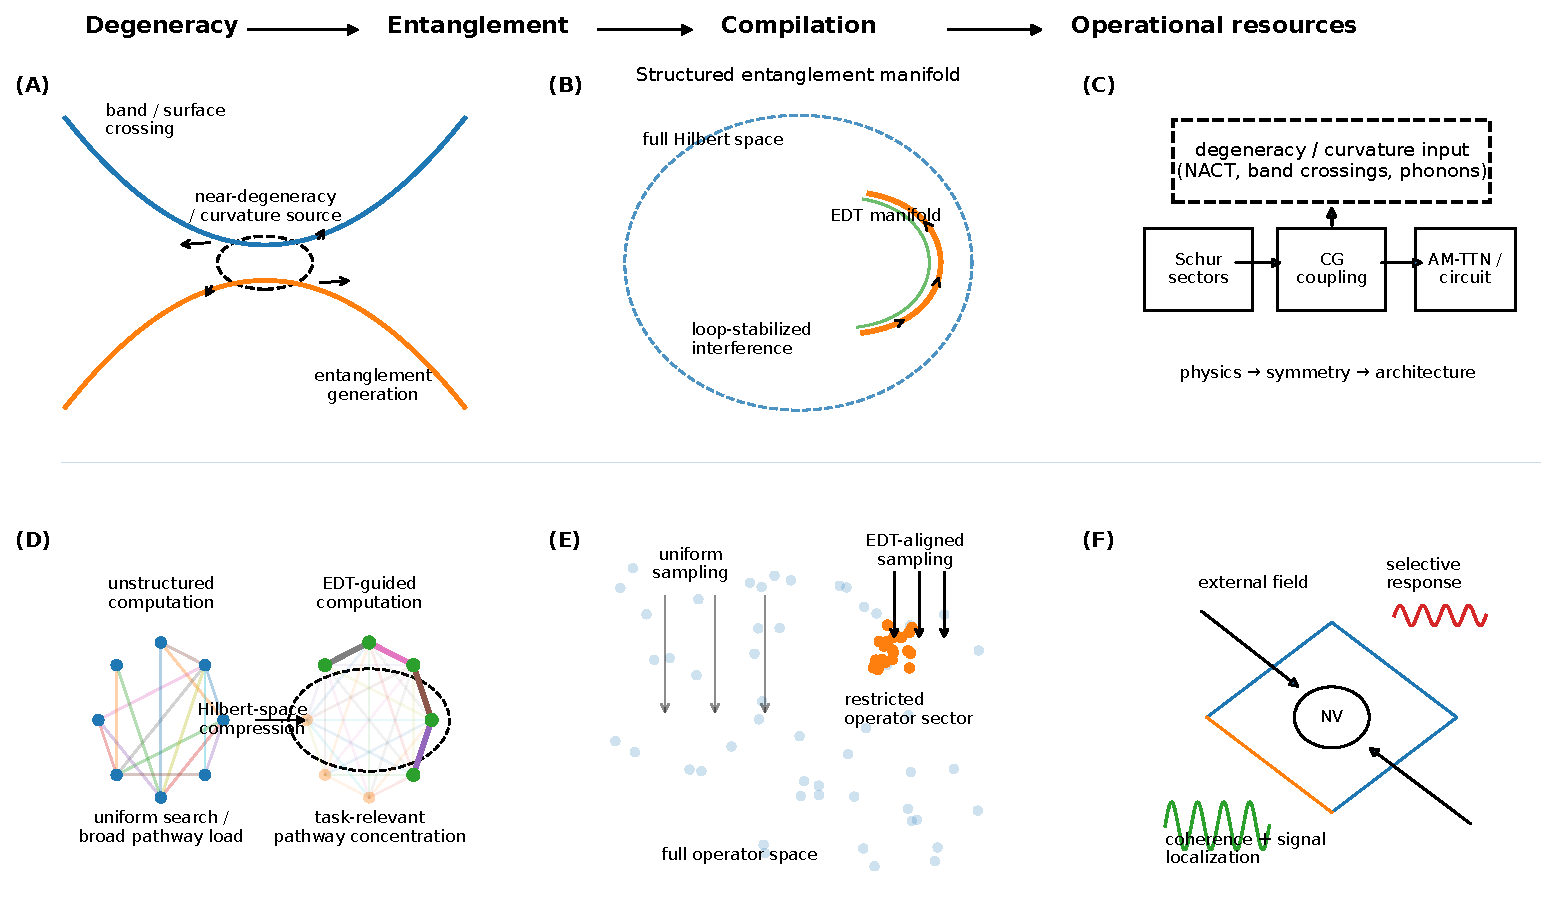
\includegraphics[width=0.92\linewidth]{fig1_edt_framework_camera_ready.pdf}
%\caption{
%\textbf{Entanglement-Dynamic Topology as a framework for programmable quantum resources.}
%(a) \textbf{Structure:} quantum states are organized by symmetry into constrained manifolds, 
%reducing the effective dimensionality of Hilbert space and concentrating accessible resources 
%into geometry-aligned subspaces.
%(b) \textbf{Interaction:} non-adiabatic coupling, particularly electron--phonon interaction, 
%generates and redistributes entanglement through modulation of electronic states and band curvature.
%(c) \textbf{Topology:} the resulting resource structure exhibits geometric organization in parameter space, 
%including nodes, poles, and vortex-like configurations that stabilize coherent interference patterns.
%(d) \textbf{Dynamics:} modulation of band energies and electronic potentials renders these structures 
%time-dependent and controllable, enabling programmable preparation and steering of resource manifolds.
%(e) \textbf{Programmable quantum resources:} together, structure, interaction, topology, and dynamics 
%define the operational regime of Entanglement-Dynamic Topology (EDT), in which entanglement, coherence, 
%superposition, and interference are localized within finite manifolds that can be compiled into 
%physical control primitives for quantum computing, sensing, and geometry-aligned algorithms.
%}
\caption{
%\textbf{Entanglement-Dynamic Topology as programmable quantum resources.}
%(a–d) EDT arises from the interplay of structure (symmetry-constrained manifolds),
%interaction (electron--phonon coupling), topology (nodes, poles, and vortices),
%and dynamics (time-dependent modulation of band energies and potentials).
%(e) These elements define a finite regime in which entanglement, coherence,
%superposition, and interference are localized within geometry-aligned manifolds
%that can be compiled into control primitives for quantum computing, sensing,
%and algorithms.
\textbf{Physical origin and organization of EDT.}
(A) Near degeneracies and band crossings act as curvature sources, where non-adiabatic coupling generates entanglement. 
(B) Structured entanglement manifold embedded within the full Hilbert space, stabilized by loop-induced interference. 
(C) Compilation of physical structure into symmetry-adapted architectures, including Schur sectors, Clebsch–Gordan coupling, and circuit representations. 
(D) Comparison between unstructured Hilbert-space exploration and EDT-guided computation, illustrating pathway concentration and effective compression. 
(E) Sampling strategies showing restriction to task-relevant operator sectors under EDT alignment. 
(F) Operational realization in sensing platforms, where structured manifolds enable selective response and coherence localization.
}
\label{fig:edt_concept}
\end{figure*}

\begin{figure*}[t]
\centering
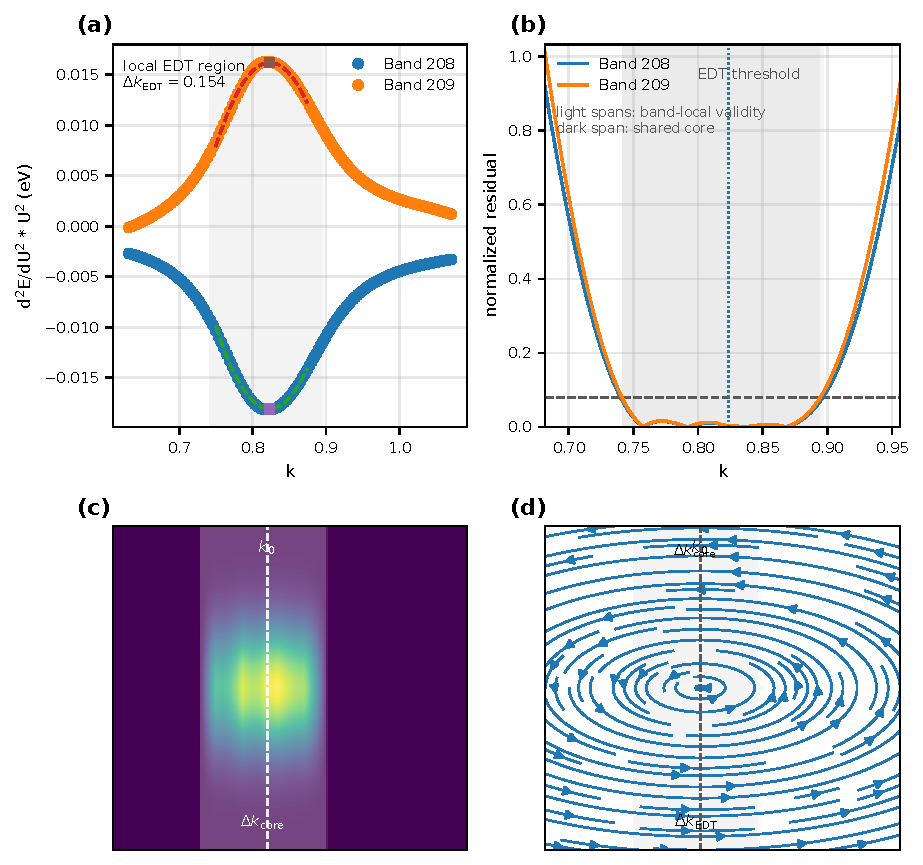
\includegraphics[width=0.92\linewidth]{fig_S7_NACT_K3C60_EDT_localfit_datamap.pdf}
\caption{
%\textbf{Data-driven identification of the Entanglement-Dynamic Topology (EDT) regime in K$_3$C$_{60}$.}
%(a) Electronic band structure along a high-symmetry path, showing paired bands in the vicinity of the Fermi level.
%(b) Curvature of band energies with respect to the control coordinate, revealing regions of enhanced second-order response associated with non-adiabatic coupling.
%(c) Local quadratic fits to paired curvature branches near the crossing region, demonstrating the emergence of a consistent effective curvature scale $k_0$ within a finite interval.
%(d) Extracted EDT window $\Delta k_{\mathrm{EDT}}$, defined as the momentum region over which the paired curvature branches admit a stable local quadratic description. Together, these panels establish an operational criterion for EDT: a finite momentum-space regime in which curvature structure is coherent, paired, and locally quadratic, indicating the presence of structured, interacting, topological, and dynamical quantum resources.
\textbf{Data-driven identification of the EDT regime in K$_3$C$_{60}$.}
(a) Curvature of band energies near a crossing, showing localized regions of enhanced second-order response. 
(b) Residual analysis defining the validity of local quadratic fits for paired curvature branches. 
(c) Local quadratic structure characterized by an intrinsic scale $k_0$ and a core region $\Delta k_{\mathrm{core}}$. 
(d) Definition of the EDT window $\Delta k_{\mathrm{EDT}}$, the finite momentum interval over which paired curvature branches remain coherent and admit a stable quadratic description. 
This window defines a data-driven criterion for identifying structured quantum resource manifolds in real materials.
}
\label{fig:k3c60_edt}
\end{figure*}


\begin{figure*}[t]
  \centering
  \includegraphics[width=0.98\linewidth]{figs/figure3_edt_regime_panel.pdf}
\caption{\textbf{Finite EDT regime from loop-controlled dynamics.}
(a) OTOC map $C_{\mathrm{OTOC}}(t,\lambda)$ showing loop-induced operator spreading. 
(b) Alignment of OTOC amplitude summaries with the long-time correlator $C_\infty$. While operator spreading increases with loop strength, $C_\infty$ decreases at large $\lambda$, and their overlap defines a finite EDT window. 
(c) OTOC time-structure metrics demonstrating temporally organized dynamics within the same interval. 
(d) Combined EDT phase score, which exhibits a clear maximum at intermediate loop strength. 
(e) Phase classification separating local, EDT, and overdriven regimes. 
(f) Scaling of the optimal loop strength $\lambda^\star$ under variation of $h_x$, demonstrating robustness of the EDT regime.
        }
  \label{fig:fig3_edt_regime}
\end{figure*}


\begin{figure*}[t]
  \centering
  \includegraphics[width=0.80\linewidth]{figs/demo_edt_gyro_trotter_4q_plaquette_otoc.pdf}
\caption{\textbf{Scaling, complexity, and hardware relevance of the EDT regime from 4-qubit plaquette Trotter realization of the EDT gyroscope model.}
(a) Optimal loop strength $\lambda^\star$ under variation of the transverse field $h_x$, showing that the EDT regime is stable over a finite parameter range. 
(b) Peak EDT score $S^\star_{\mathrm{EDT}}$, which exhibits non-monotonic dependence on $h_x$, reflecting competition between operator spreading and long-time correlation. 
(c) Circuit depth and gate count versus evolution time for the Trotterized implementation, showing predictable scaling. 
(d) Observable and OTOC errors versus time, demonstrating that approximation errors remain controlled in the relevant regime. 
(e) Optimal loop strength $\lambda^\star$ versus Trotter budget, showing insensitivity to compilation depth. 
(f) Peak EDT score versus Trotter budget, demonstrating robustness of the EDT regime under approximate circuit implementation.
	}
  \label{fig:si_4q_plaquette_trotter}
\end{figure*}

\begin{figure*}[t]
  \centering
  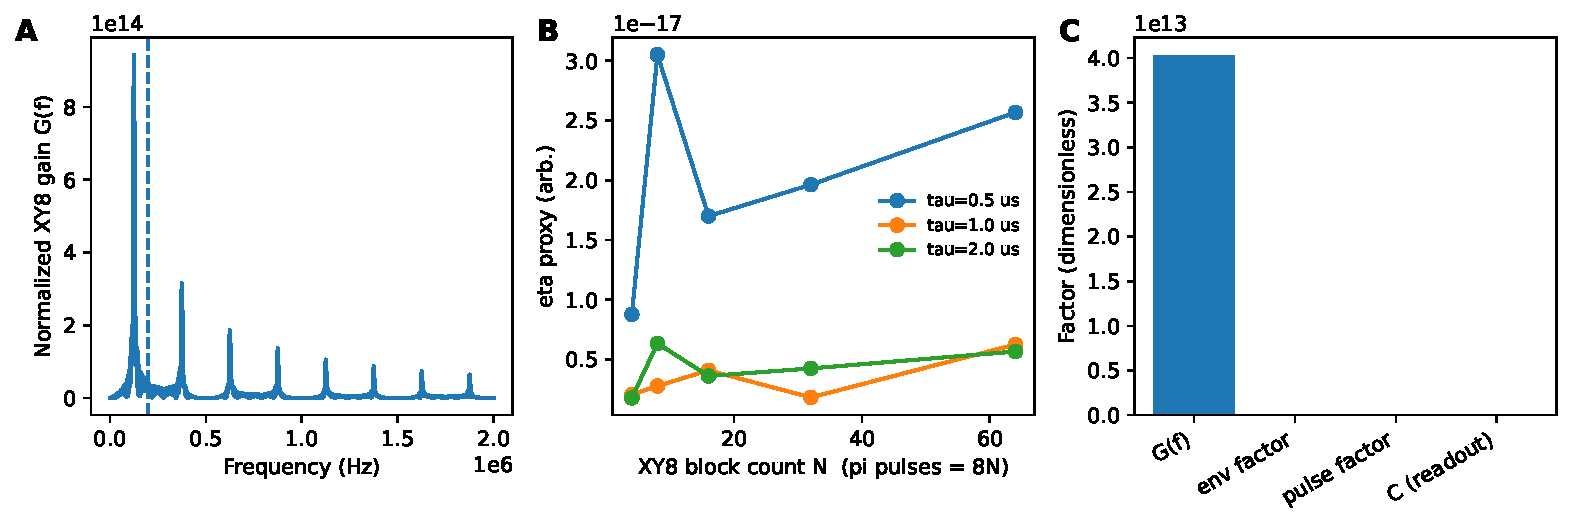
\includegraphics[width=0.90\linewidth]{figs/fig_xy8_qre_nv.pdf}
\caption{\textbf{Quantum resource engineering in NV-center sensing.}
(A) Filter response function $G(f)$ for an XY8 sequence, showing frequency-selective amplification. 
(B) Sensitivity proxy as a function of pulse number $N$ and spacing $\tau$, demonstrating a finite optimal regime. 
(C) Decomposition of sensing performance into resource factors, including filter gain, environmental coherence, pulse fidelity, and readout contrast. 
These results show that optimal sensing arises from a structured balance of competing quantum resources, providing an experimental realization of the EDT regime.
        }
  \label{fig:fig5_nvdemo}
\end{figure*}

%\begin{figure*}[t]
%  \centering
%  \includegraphics[width=0.62\textwidth]{figs/demo_edt_gyro_trotter_4q_circuit_example.pdf}
%\caption{\textbf{4-qubit plaquette Trotter realization of the EDT gyroscope toy model.}
%\textbf{Bottom,} Representative first-order Qiskit Trotter circuit for the four-qubit plaquette model.}
%  \label{fig:si_4q_plaquette_trotter_circuits}
%\end{figure*}

%\section*{Figure Index}

%\textbf{Main Text Figures}

%\begin{itemize}
%\item \textbf{Figure 1:} Conceptual framework of Entanglement--Dynamic Topology (EDT), illustrating the roles of symmetry, interaction, topology, and dynamics.
%\item \textbf{Figure 2:} Data-driven identification of the EDT regime in K$_3$C$_{60}$ via curvature-resolved band structure.
%\item \textbf{Figure 3:} Emergence of the EDT regime in a minimal dynamical model, showing structured operator spreading and persistent correlations.
%\item \textbf{Figure 4:} Scaling and implementation analysis, demonstrating robustness of the EDT regime under circuit approximations.
%\item \textbf{Figure 5:} Experimental realization of the EDT principle in NV-center sensing, showing finite optimal regimes in control space.
%\end{itemize}
%
%\vspace{1em}
%
%\textbf{Supplementary Figures}
%
%\begin{itemize}
%\item \textbf{Figure S1:} Curvature and degeneracy removal in Na.
%\item \textbf{Figure S2:} Curvature structure in V.
%\item \textbf{Figure S3:} Extended curvature structures defining the EDT regime in K$_3$C$_{60}$.
%\item \textbf{Figure S4:} Anisotropic curvature structures in YBa$_2$Cu$_3$O$_7$.
%\item \textbf{Figure S5:} Strong curvature response in LaH$_{10}$.
%\item \textbf{Figure S6:} Temperature-dependent band structure and degeneracy lifting in Nb.
%\end{itemize}
%\bibliographystyle{unsrt}
%\bibliography{references}

\end{document}
